\documentclass[11pt,a4paper,oneside]{report}

\usepackage[utf8]{inputenc}
\usepackage[T1]{fontenc}
\usepackage[italian]{babel}
\usepackage{lmodern}
\usepackage{microtype}
\usepackage{graphicx}
\usepackage{caption}
\captionsetup{font={small,sf}, labelfont=bf}
\usepackage[top=2.5cm, bottom=2.5cm, left=2.5cm, right=2.5cm]{geometry}

\usepackage{amsmath,amssymb,amsthm,mathtools,bm}
\usepackage{booktabs}
\usepackage{tabularx}
\usepackage{array}
\usepackage{enumitem}
\usepackage{fancyhdr}
\usepackage{titlesec}
\usepackage{xcolor}
\usepackage{float}
\usepackage[most]{tcolorbox}
\usepackage{tikz}
\usetikzlibrary{arrows.meta, patterns, calc, shapes.geometric}

\usepackage[colorlinks=true,
            linkcolor=blue!80!black,
            citecolor=teal!80!black,
            urlcolor=cyan!80!black,
            bookmarksdepth=3]{hyperref}

\definecolor{primaryBlue}{RGB}{24, 76, 120}
\definecolor{slateBg}{RGB}{248, 250, 252}
\definecolor{slateBorder}{RGB}{203, 213, 225}
\definecolor{accentGreen}{RGB}{22, 163, 74}
\definecolor{accentAmber}{RGB}{217, 119, 6}
\definecolor{accentRed}{RGB}{220, 38, 38}
\definecolor{textDark}{RGB}{15, 23, 42}
\colorlet{amber}{accentAmber}

\newtcolorbox{definizione}[1][]{
  enhanced, colback=slateBg, colframe=primaryBlue,
  fonttitle=\bfseries\sffamily, title={Definizione Fondamentale: #1},
  arc=3mm, boxrule=1pt, top=3mm, bottom=3mm, left=4mm, right=4mm
}

\newtcolorbox{leggefisica}[1][]{
  enhanced, colback=slateBg, colframe=primaryBlue,
  fonttitle=\bfseries\sffamily, title={Principio e Legge Fisica: #1},
  arc=3mm, boxrule=1pt, top=3mm, bottom=3mm, left=4mm, right=4mm
}

\newtcolorbox{commento}[1][]{
  enhanced, colback=accentAmber!5!white, colframe=accentAmber,
  fonttitle=\bfseries\sffamily, title={Interpretazione Fisica e Metodologia: #1},
  arc=3mm, boxrule=0.8pt, top=3mm, bottom=3mm, left=4mm, right=4mm
}

\newtcolorbox{avviso}[1][]{
  enhanced, colback=red!5!white, colframe=accentRed,
  fonttitle=\bfseries\sffamily, title={Attenzione al Tranello: #1},
  arc=3mm, boxrule=1pt, top=3mm, bottom=3mm, left=4mm, right=4mm
}

\newtcolorbox{metodo}[1][]{
  enhanced, breakable, colback=white, colframe=primaryBlue,
  fonttitle=\bfseries\sffamily, title={Risoluzione ed Analisi: #1},
  arc=3mm, boxrule=0.8pt, top=3mm, bottom=3mm, left=4mm, right=4mm
}

\newtcolorbox{problema}[1][]{
  enhanced, colback=white, colframe=accentGreen,
  fonttitle=\bfseries\sffamily, title={Problema Risolto: #1},
  arc=3mm, boxrule=0.8pt, top=3mm, bottom=3mm, left=4mm, right=4mm
}

\pagestyle{fancy}
\fancyhf{}
\fancyhead[L]{\small\sffamily Liceo Scientifico Statale «Leonardo da Vinci» – Maglie}
\fancyhead[R]{\small\sffamily Fisica – Classe 1B}
\fancyfoot[C]{\thepage}
\renewcommand{\headrulewidth}{0.4pt}

\titleformat{\chapter}[display]
  {\normalfont\sffamily\huge\bfseries\color{primaryBlue}}
  {\chaptertitlename\ \thechapter}{15pt}{\Huge}

\begin{document}

% Frontespizio Ufficiale
\begin{titlepage}
\begin{center}
  \vspace*{0.8cm}
  {\Large\textbf{LICEO SCIENTIFICO STATALE «LEONARDO DA VINCI»}}\\[0.25cm]
  {\large\textbf{MAGLIE (LE)}}\\[1.8cm]
  \rule{\textwidth}{1.5pt}\\[0.6cm]
  {\fontsize{24}{32}\selectfont\bfseries\color{primaryBlue} FONDAMENTI DELLA FISICA\par}\vspace{0.5cm}
  {\fontsize{12}{18}\selectfont\bfseries\color{textDark} IL METODO SPERIMENTALE, LE GRANDEZZE FONDAMENTALI,\\[0.15cm] LA TEORIA DELLE PROPORZIONI, LE RELAZIONI CARTESIANE\\[0.15cm] ED IL PRONTUARIO DELLE FORMULE INVERSE\par}\vspace{0.5cm}
  \rule{\textwidth}{1.5pt}\\[2cm]
  
  \begin{minipage}{0.48\textwidth}
    \textbf{Docente:}\\
    Prof. Giuseppe De Pascali\\
    \textit{Dipartimento di Matematica e Fisica}
  \end{minipage}
  \hfill
  \begin{minipage}{0.48\textwidth}
    \raggedleft
    \textbf{Classe:}\\
    1ª Sezione B\\
    \textit{Liceo Scientifico Tradizionale}\\
    Anno Scolastico 2026/2027
  \end{minipage}

  \vfill
  {\small Monografia Didattica Completa con Spiegazioni Dettagliate, Teoria degli Errori e Schemi Vettoriali TikZ (Standard Master 4.0)}
\end{center}
\end{titlepage}

\tableofcontents
\newpage

\chapter{Il Metodo Scientifico Sperimentale e le Grandezze Fisiche}

\section{La Rivoluzione Galileiana e il Metodo Sperimentale}
La fisica contemporanea nasce nel XVII secolo grazie all'opera di \textbf{Galileo Galilei}, che supera la visione speculativa e qualitativa della filosofia aristotelica introducendo il \textbf{metodo sperimentale} (o scientifico). 
La comprensione della natura non può basarsi sul principio di autorità (\textit{ipse dixit}), né su argomentazioni puramente dialettiche, ma sull'interrogazione metodica e rigorosa della realtà materiale.

Il metodo sperimentale si articola in quattro tappe inscindibili e ricorsive:
\begin{enumerate}[label=\textbf{\arabic*.}]
  \item \textbf{Osservazione sistematica del fenomeno:} identificazione di un evento naturale e isolamento dei parametri rilevanti, eliminando le circostanze secondarie o contingenti;
  \item \textbf{Formulazione di un'ipotesi matematica:} elaborazione di un modello concettuale provvisorio espresso in forma di equazioni o relazioni funzionali tra grandezze;
  \item \textbf{Cimento o Verifica Sperimentale (Esperimento di Laboratorio):} riproduzione controllata del fenomeno in condizioni artificiali prestabilite (\textit{ceteris paribus}, ossia facendo variare un solo parametro alla volta mantenendo costanti tutti gli altri). Se i dati sperimentali smentiscono l'ipotesi, essa viene rigettata o corretta;
  \item \textbf{Enunciazione della Legge Fisica Universale:} formalizzazione matematica della legge generale che descrive e prevede il comportamento di tutti i sistemi fisici analoghi, valida fino a un eventuale esperimento falsificante.
\end{enumerate}

\section{Definizione Operativa di una Grandezza Fisica}
Nel linguaggio scientifico, non tutte le proprietà di un corpo o di un evento sono indagabili dalla fisica. 
Sentimenti, preferenze estetiche o qualità puramente soggettive non possono essere trattate quantitativamente.

\begin{definizione}[Grandezza Fisica e Definizione Operativa]
Una proprietà della materia o di un fenomeno naturale è una \textbf{grandezza fisica} se e solo se per essa è stabilita una \textbf{definizione operativa}, la quale prescrive:
\begin{enumerate}[label=\alph*)]
  \item La procedura sperimentale oggettiva e ripetibile con cui effettuare la misurazione;
  \item La scelta di un'opportuna \textbf{unità di misura omogenea} e l'impiego di uno strumento campione tarato.
\end{enumerate}
Misurare una grandezza fisica significa determinare il rapporto numerico tra la grandezza in esame e l'unità di misura assunta come riferimento:
\[
\text{Grandezza Misurata } x = \{x\} \cdot [u]
\]
dove $\{x\} \in \mathbb{R}$ rappresenta la misura scalare (il numero) e $[u]$ è l'unità di misura prescelta.
\end{definizione}

\begin{commento}[Grandezze Intensive ed Estensive]
Una fondamentale distinzione termodinamica e meccanica tra grandezze fisiche è la seguente:
\begin{itemize}
  \item \textbf{Grandezze Estensive:} dipendono direttamente dall'estensione o dalla quantità di materia del sistema considerato. Esse godono della proprietà additiva (es. massa $m$, volume $V$, lunghezza $l$, carica elettrica $Q$, energia interna $U$).
  \item \textbf{Grandezze Intensive:} sono indipendenti dalla quantità di materia e descrivono lo stato locale del corpo in ogni suo punto infinitesimo (es. temperatura $T$, pressione $p$, densità volumica $\rho = m/V$, calore specifico $c_s$).
\end{itemize}
\end{commento}

\section{Il Sistema Internazionale di Unità di Misura (SI)}
Per assicurare l'universalità delle comunicazioni scientifiche ed eliminare ambiguità metrologiche, nel 1960 la Conferenza Generale dei Pesi e delle Misure ha istituito il \textbf{Sistema Internazionale di Unità (SI)}, fondato su \textbf{sette grandezze fondamentali}:

\begin{table}[htbp]
\centering
\small
\renewcommand{\arraystretch}{1.25}
\begin{tabularx}{\textwidth}{llllX}
\toprule
\textbf{Grandezza Fondamentale} & \textbf{Simbolo} & \textbf{Unità SI} & \textbf{Simbolo} & \textbf{Costante Universale di Riferimento (Def. 2019)} \\
\midrule
Lunghezza & $l, s, d$ & metro & $\text{m}$ & Velocità della luce nel vuoto ($c = 299\,792\,458\,\text{m/s}$) \\
Massa & $m$ & chilogrammo & $\text{kg}$ & Costante di Planck ($h = 6{,}626\,070\,15 \cdot 10^{-34}\,\text{J}\cdot\text{s}$) \\
Intervallo di Tempo & $t, \tau$ & secondo & $\text{s}$ & Transizione iperfine del cesio-133 ($\Delta\nu_{\text{Cs}}$) \\
Intensità di Corrente & $I, i$ & ampere & $\text{A}$ & Carica elementare ($e = 1{,}602\,176\,634 \cdot 10^{-19}\,\text{C}$) \\
Temperatura Termodinamica & $T$ & kelvin & $\text{K}$ & Costante di Boltzmann ($k_B = 1{,}380\,649 \cdot 10^{-23}\,\text{J/K}$) \\
Quantità di Sostanza & $n$ & mole & $\text{mol}$ & Costante di Avogadro ($N_A = 6{,}022\,140\,76 \cdot 10^{23}\,\text{mol}^{-1}$) \\
Intensità Luminosa & $I_v$ & candela & $\text{cd}$ & Efficacia luminosa monocromatica ($K_{\text{cd}}$) \\
\bottomrule
\end{tabularx}
\caption{Le sette grandezze fondamentali del Sistema Internazionale (SI).}
\label{tab:grandezze_si}
\end{table}

Tutte le altre grandezze fisiche (es. velocità $v = s/t$, forza $F = m \cdot a$, pressione $p = F/S$, energia e lavoro $W = F \cdot s$) sono \textbf{grandezze derivate}, ottenute combinando algebricamente le grandezze fondamentali mediante le rispettive definizioni fisiche.

\section{Notazione Scientifica, Prefissi e Ordini di Grandezza}
Nel mondo microscopico e cosmico, le misure fisiche spaziano su scale enormi: dal raggio del protone ($\approx 10^{-15}\,\text{m}$) alla distanza delle galassie remote ($\approx 10^{26}\,\text{m}$). Per evitare scritture ingombranti con decine di zeri, la fisica impiega sistematicamente la \textbf{notazione scientifica}.

\begin{definizione}[Notazione Scientifica]
Un numero reale positivo $N$ è scritto in \textbf{notazione scientifica} quando si presenta nella forma:
\[
N = m \cdot 10^p \qquad \text{con } 1 \le m < 10 \quad \text{e} \quad p \in \mathbb{Z}
\]
dove $m$ è detto \textbf{mantissa} (o coefficiente significativo) e $p$ è l'\textbf{esponente intero} (potenza di dieci).
\end{definizione}

\begin{definizione}[Ordine di Grandezza]
L'\textbf{ordine di grandezza} di un numero positivo $N = m \cdot 10^p$ è la potenza di dieci più vicina al numero stesso:
\begin{itemize}
  \item Se $1 \le m < \sqrt{10} \approx 3{,}162$, l'ordine di grandezza è $\mathbf{10^p}$;
  \item Se $3{,}162 \le m < 10$, l'ordine di grandezza è $\mathbf{10^{p+1}}$.
\end{itemize}
\end{definizione}

\begin{commento}[Esempi di Conversione e Calcolo di Ordine di Grandezza]
\begin{itemize}
  \item Durata di un anno terrestre: $T = 365 \cdot 24 \cdot 3600\,\text{s} = 31\,536\,000\,\text{s} = 3{,}1536 \cdot 10^7\,\text{s}$. Poiché $3{,}1536 < 3{,}162$, l'ordine di grandezza è $10^7\,\text{s}$.
  \item Raggio equatoriale terrestre: $R_\oplus \approx 6\,378\,000\,\text{m} = 6{,}378 \cdot 10^6\,\text{m}$. Poiché $6{,}378 > 3{,}162$, l'ordine di grandezza è $10^7\,\text{m}$.
\end{itemize}
\end{commento}

\chapter{Gli Strumenti di Misura e la Bilancia a Bracci Uguali}

\section{Caratteristiche Metrologiche degli Strumenti}
Ogni strumento di misura, sia esso analogico (con indice e scala graduata) o digitale (con display elettronico), possiede proprietà metrologiche essenziali che ne determinano l'applicabilità e i limiti operativi:
\begin{itemize}
  \item \textbf{Portata (Fondo Scala):} il valore massimo della grandezza fisica che lo strumento è in grado di misurare senza subire danni meccanici o saturazione del segnale;
  \item \textbf{Sensibilità (Risoluzione):} la minima variazione della grandezza misurata capace di provocare un movimento apprezzabile dell'indice o un incremento dell'ultima cifra sul quadrante;
  \item \textbf{Prontezza:} l'intervallo temporale necessario affinché lo strumento fornisca la lettura definitiva stabile dopo essere stato sollecitato;
  \item \textbf{Precisione (Ripetibilità):} l'attitudine dello strumento a fornire misure molto vicine tra loro quando ripetute nelle medesime condizioni sperimentali;
  \item \textbf{Accuratezza:} la capacità dello strumento di fornire una lettura coincidente con il valore convenzionalmente vero del campione tarato.
\end{itemize}

\section{La Bilancia a Bracci Uguali: Teoria Meccanica ed Equilibrio Statico}
La \textbf{bilancia a bracci uguali} è uno dei più antichi e perfetti strumenti di misura della fisica. Essa consente la misura diretta della \textbf{massa inerziale e gravitazionale} di un corpo mediante il metodo di \textbf{confronto diretto} (o azzeramento) con masse campione tarate.

\subsection{Architettura Meccanica}
Lo strumento è costituito da:
\begin{enumerate}
  \item Un \textbf{giogo rigido orizzontale} di massa ridotta e indeformabile, capace di oscillare attorno a un fulcro centrale;
  \item Un \textbf{fulcro a coltello} (prismatico, in agata dura o acciaio speciale) appoggiato su un piano orizzontale levigato per ridurre al minimo l'attrito radente;
  \item Due \textbf{bracci} rigorosamente simmetrici e di eguale lunghezza $b_1 = b_2 = b$;
  \item Due \textbf{piatti di pesata} sospesi alle estremità dei bracci tramite staffe flessibili;
  \item Un \textbf{indice centrale (ago)} solidale al giogo e perpendicolare ad esso, la cui estremità scorre davanti a una \textbf{scala graduata con zero centrale}.
\end{enumerate}

\subsection{Condizione Fisica di Equilibrio dei Momenti Torcenti}
Consideriamo una massa incognita $m_x$ posizionata sul piatto sinistro e una massa nota di confronto $m_0$ posizionata sul piatto destro. 
Su ciascun piatto agisce la rispettiva forza peso diretta verticalmente verso il basso:
\[
\vec{F}_{p,x} = m_x \cdot \vec{g}, \qquad \vec{F}_{p,0} = m_0 \cdot \vec{g}
\]
dove $\vec{g}$ rappresenta l'accelerazione di gravità locale.
La condizione necessaria e sufficiente affinché il giogo si mantenga in perfetto equilibrio statico orizzontale (indice perfettamente sullo zero centrale) è che la risultante dei momenti torcenti delle forze applicate rispetto al fulcro sia nulla:
\[
\sum \vec{M}_O = \vec{0} \implies M_{\text{sinistro}} = M_{\text{destro}}
\]
Esplicitando i moduli dei momenti (forza per braccio):
\[
F_{p,x} \cdot b = F_{p,0} \cdot b \iff (m_x \cdot g) \cdot b = (m_0 \cdot g) \cdot b
\]
Semplificando la lunghezza comune del braccio $b > 0$:
\[
m_x \cdot g = m_0 \cdot g
\]
Poiché l'accelerazione di gravità locale $g$ agisce in modo rigorosamente identico su entrambi i piatti, possiamo dividere ambo i membri per $g \neq 0$:
\[
\mathbf{m_x = m_0}
\]

\begin{figure}[htbp]
\centering
\begin{tikzpicture}[scale=0.95, >=stealth]
  % Basamento massiccio
  \fill[gray!25, draw=gray!70, thick] (1.0, 0) rectangle (7.0, 0.4);
  \node[font=\footnotesize, color=gray!80!black] at (4.0, 0.2) {Basamento Antivibrante Livellato};

  % Colonna centrale verticale
  \fill[gray!40, draw=gray!80, thick] (3.8, 0.4) rectangle (4.2, 3.8);

  % Scala graduata centrale ad arco con zero
  \draw[thick, slateBorder] (3.2, 1.2) arc (200:340:0.85);
  \foreach \angle in {210, 230, 250, 270, 290, 310, 330} {
    \draw[gray!70, thin] ({4.0 + 0.85*cos(\angle)}, {1.9 + 0.85*sin(\angle)}) -- ({4.0 + 0.72*cos(\angle)}, {1.9 + 0.72*sin(\angle)});
  }
  \node[font=\tiny, primaryBlue, font=\bfseries] at (4.0, 0.8) {Zero di Equilibrio};
  \fill[accentRed] (4.0, 1.05) circle (1.5pt);

  % Fulcro centrale a coltello (triangolo)
  \fill[accentAmber!80!black] (3.85, 3.8) -- (4.15, 3.8) -- (4.0, 4.05) -- cycle;
  \node[above, font=\scriptsize, accentAmber!80!black] at (4.0, 4.15) {Fulcro $O$};

  % Giogo orizzontale perfettamente in bolla
  \draw[line width=3.5pt, primaryBlue] (1.2, 4.05) -- (6.8, 4.05);

  % Ago indice verticale puntato sullo zero
  \draw[very thick, accentRed] (4.0, 4.05) -- (4.0, 1.15);
  \fill[accentRed] (4.0, 4.05) circle (3pt);

  % Quote bracci b1 e b2 con nodi protetti da cuscino opaco
  \draw[<->, thick, primaryBlue!80] (1.2, 4.5) -- (4.0, 4.5) 
    node[midway, fill=white, fill opacity=0.9, text opacity=1, inner sep=1.5pt, font=\small\bfseries] {Braccio sinistro $b$};
  \draw[<->, thick, primaryBlue!80] (4.0, 4.5) -- (6.8, 4.5) 
    node[midway, fill=white, fill opacity=0.9, text opacity=1, inner sep=1.5pt, font=\small\bfseries] {Braccio destro $b$};

  % Fili di sospensione piatti
  \draw[thick, gray!80] (1.2, 4.05) -- (0.5, 2.2) -- (1.9, 2.2) -- cycle;
  \draw[thick, gray!80] (6.8, 4.05) -- (6.1, 2.2) -- (7.5, 2.2) -- cycle;

  % Piatti di pesata
  \fill[primaryBlue!15, draw=primaryBlue, thick] (0.4, 2.1) rectangle (2.0, 2.25);
  \fill[primaryBlue!15, draw=primaryBlue, thick] (6.0, 2.1) rectangle (7.6, 2.25);

  % Massa incognita mx sul piatto sinistro
  \fill[accentGreen!30, draw=accentGreen!80!black, thick] (0.8, 2.25) rectangle (1.6, 3.1);
  \node[font=\footnotesize\bfseries, accentGreen!80!black] at (1.2, 2.68) {Massa $m_x$};

  % Masse campioni note m0 sul piatto destro
  \fill[primaryBlue!30, draw=primaryBlue, thick] (6.35, 2.25) rectangle (7.25, 2.85);
  \fill[primaryBlue!40, draw=primaryBlue, thick] (6.55, 2.85) rectangle (7.05, 3.25);
  \node[font=\footnotesize\bfseries, primaryBlue] at (6.8, 2.55) {Campioni $m_0$};

  % Vettori forze peso verso il basso
  \draw[->, line width=1.5pt, accentGreen!80!black] (1.2, 2.1) -- (1.2, 0.9)
    node[right, font=\footnotesize\bfseries, fill=white, fill opacity=0.9, text opacity=1, inner sep=1pt] {$\vec{F}_{p,x} = m_x \vec{g}$};
  \draw[->, line width=1.5pt, primaryBlue] (6.8, 2.1) -- (6.8, 0.9)
    node[right, font=\footnotesize\bfseries, fill=white, fill opacity=0.9, text opacity=1, inner sep=1pt] {$\vec{F}_{p,0} = m_0 \vec{g}$};

  % Didascalia algebrica di equilibrio
  \node[below, font=\small\bfseries, primaryBlue] at (4.0, -0.2) 
    {Condizione di Equilibrio dei Momenti: $\sum M = 0 \iff m_x \cdot g \cdot b = m_0 \cdot g \cdot b \implies m_x = m_0$};
\end{tikzpicture}
\caption{Schema meccanico analitico della bilancia a bracci uguali in equilibrio statico.}
\label{fig:bilancia_bracci_uguali}
\end{figure}

\subsection{Indipendenza Rigorosa dall'Accelerazione di Gravità $g$}
Un'evidenza concettuale straordinaria differenzia la \textbf{bilancia a bracci uguali} dal \textbf{dinamometro a molla}:
\begin{leggefisica}[Invarianza Gravitazionale della Bilancia a Bracci Uguali]
La bilancia a bracci uguali confronta direttamente due masse mediante l'annullamento della risultante dei momenti. 
Poiché il fattore $g$ compare a moltiplicare sia al primo sia al secondo membro, esso si elide identicamente. 
Ne consegue che:
\textbf{Se una bilancia a bracci uguali è in equilibrio sulla superficie terrestre, essa resterà in perfetto equilibrio sulla Luna, su Marte o all'interno di una stazione spaziale orbitante soggetta a gravità ridotta.}
Al contrario, il dinamometro misura la forza peso $F_p = m \cdot g$: sulla Luna la medesima massa allungherebbe la molla di una frazione pari a circa $1/6$ rispetto alla Terra ($g_{\text{luna}} \approx 1{,}62\,\text{m/s}^2$).
\end{leggefisica}

\chapter{Teoria della Misura, Incertezze e Propagazione degli Errori}

\section{L'Inevitabilità dell'Incertezza Sperimentale}
In fisica sperimentale è assiomatico che \textbf{non esiste la misura esatta}: qualsiasi atto di misurazione è inesorabilmente accompagnato da un margine di indeterminazione, detto \textbf{incertezza di misura} (o errore sperimentale).
Gli errori di misura si classificano rigorosamente in due grandi categorie:

\begin{enumerate}
  \item \textbf{Errori Sistematici:} agiscono sempre nello stesso verso (per eccesso o per difetto) e con la medesima intensità ogni volta che si ripete la misura.
  \textit{Cause tipiche:} difetto di taratura dello strumento (es. indice non azzerato), deterioramento meccanico, errore di parallasse dell'operatore, variazioni ambientali non compensate.
  \textit{Proprietà didattica:} gli errori sistematici possono essere individuati, corretti o rimossi mediante opportuna ritaratura dello strumento o raffinamento della procedura.
  \item \textbf{Errori Casuali (o Accidentali):} sono fluttuazioni imprevedibili, causate da una miriade di fattori microscopici incontrollabili (correnti d'aria, microvibrazioni del banco, impercettibili esitazioni nei riflessi umani al cronometro). Essi agiscono sia per eccesso sia per difetto con pari probabilità statistica.
  \textit{Proprietà didattica:} gli errori casuali non possono essere eliminati, ma possono essere minimizzati e quantificati statisticamente ripetendo la misura molteplici volte.
\end{enumerate}

\section{Valore Attendibile e Incertezza Assoluta}
Quando si misura una grandezza fisica $x$, il modo di stimare il \textbf{valore attendibile} $\bar{x}$ e l'\textbf{incertezza assoluta} $\Delta x$ dipende dal numero di misurazioni effettuate:

\subsection{Misura Singola}
Nel caso di una singola misura, il valore attendibile coincide con il valore letto sullo strumento, mentre l'incertezza assoluta $\Delta x$ si assume convenzionalmente pari alla \textbf{sensibilità dello strumento}:
\[
\bar{x} = x_{\text{letto}}, \qquad \Delta x = \text{Sensibilità dello strumento}
\]

\subsection{Serie di Misure Ripetute ($N$ prove)}
Se la misura viene ripetuta $N$ volte nelle stesse condizioni ($x_1, x_2, \dots, x_N$):
\begin{enumerate}
  \item Il \textbf{valore attendibile} è la \textbf{media aritmetica} dei valori:
  \[
  \bar{x} = \frac{1}{N} \sum_{i=1}^N x_i = \frac{x_1 + x_2 + \dots + x_N}{N}
  \]
  \item L'\textbf{incertezza assoluta} (per serie brevi, tipiche della didattica liceale) è la \textbf{semidispersione massima}:
  \[
  \Delta x = \frac{x_{\max} - x_{\min}}{2}
  \]
  \textit{Clausola di garanzia metrologica:} se il valore calcolato per la semidispersione massima risulta inferiore alla sensibilità dello strumento impiegato, si assume inderogabilmente come incertezza assoluta la \textbf{sensibilità dello strumento}:
  \[
  \Delta x = \max\left(\frac{x_{\max} - x_{\min}}{2}, \; \text{Sensibilità}\right)
  \]
\end{enumerate}

\begin{definizione}[Scrittura Standard del Risultato di Misura]
Il risultato finale di una misurazione si esprime formalmente indicando il valore attendibile affiancato dall'incertezza assoluta e dall'unità di misura:
\[
x = (\bar{x} \pm \Delta x)\;[u]
\]
Tale espressione indica che il valore "vero" della grandezza fisica $x_{\text{vero}}$ appartiene con elevata probabilità all'\textbf{intervallo di confidenza}:
\[
\bar{x} - \Delta x \le x_{\text{vero}} \le \bar{x} + \Delta x
\]
\end{definizione}

\begin{figure}[htbp]
\centering
\begin{tikzpicture}[scale=1.1, >=stealth]
  % Asse dei valori misurati
  \draw[->, thick, primaryBlue] (0, 0) -- (9, 0) node[right, font=\small] {$x\;[u]$};

  % Valore centrale media
  \draw[very thick, primaryBlue] (4.5, -0.3) -- (4.5, 0.3) 
    node[above, fill=white, fill opacity=0.9, text opacity=1, inner sep=2pt, font=\bfseries] {Valore attendibile $\bar{x}$};
  \fill[primaryBlue] (4.5, 0) circle (3pt);

  % Intervallo di incertezza campito
  \fill[accentGreen!20, draw=accentGreen, thick] (2.2, -0.2) rectangle (6.8, 0.2);

  % Estremi intervallo
  \draw[thick, accentGreen!80!black] (2.2, -0.35) -- (2.2, 0.35)
    node[below=4pt, fill=white, fill opacity=0.9, text opacity=1, inner sep=1.5pt, font=\small] {$\bar{x} - \Delta x$};
  \draw[thick, accentGreen!80!black] (6.8, -0.35) -- (6.8, 0.35)
    node[below=4pt, fill=white, fill opacity=0.9, text opacity=1, inner sep=1.5pt, font=\small] {$\bar{x} + \Delta x$};

  % Frecce quota semi-ampiezza Delta x
  \draw[<->, thick, accentAmber!90!black] (2.2, 0.6) -- (4.5, 0.6) 
    node[midway, above, fill=white, fill opacity=0.9, text opacity=1, inner sep=1pt, font=\footnotesize\bfseries] {$\Delta x$};
  \draw[<->, thick, accentAmber!90!black] (4.5, 0.6) -- (6.8, 0.6) 
    node[midway, above, fill=white, fill opacity=0.9, text opacity=1, inner sep=1pt, font=\footnotesize\bfseries] {$\Delta x$};

  % Nodo intervallo di confidenza
  \node[font=\footnotesize, color=gray!80!black] at (4.5, -0.85) 
    {Intervallo di Incertezza $[\bar{x} - \Delta x, \; \bar{x} + \Delta x]$ di ampiezza $2\Delta x$};
\end{tikzpicture}
\caption{Rappresentazione geometrica dell'intervallo di confidenza di una misura fisica.}
\label{fig:intervallo_incertezza}
\end{figure}

\section{Errore Relativo ed Errore Percentuale}
L'incertezza assoluta $\Delta x$, pur essendo fondamentale, non fornisce informazioni sulla \textbf{qualità intrinseca della misurazione}. 
Infatti, commettere un errore assoluto di $\Delta x = 1\,\text{cm}$ nel misurare la lunghezza di una penna di $10\,\text{cm}$ rappresenta una misura assai grossolana (errore del 10\%); lo stesso errore di $1\,\text{cm}$ nel misurare la lunghezza di un campo di atletica di $100\,\text{m} = 10\,000\,\text{cm}$ rappresenta invece una misurazione di straordinaria accuratezza (errore dello 0{,}01\%).

\begin{definizione}[Errore Relativo ed Errore Percentuale]
Si definisce \textbf{errore relativo} $e_r$ il rapporto tra l'incertezza assoluta e il valore attendibile della misura:
\[
\mathbf{e_r = \frac{\Delta x}{\bar{x}}}
\]
L'errore relativo è un \textbf{numero puro adimensionale} (privo di unità di misura). 
Moltiplicando l'errore relativo per cento si ottiene l'\textbf{errore percentuale} $e_p$:
\[
\mathbf{e_p = e_r \cdot 100\% = \left(\frac{\Delta x}{\bar{x}}\right) \cdot 100\%}
\]
L'errore percentuale misura oggettivamente la precisione della misura: tanto più $e_p$ è ridotto, tanto più la misura è accurata.
\end{definizione}

\section{Propagazione delle Incertezze nelle Misure Indirette}
Quando una grandezza fisica $z$ non viene misurata direttamente con uno strumento, ma viene ricavata combinando algebricamente altre misure sperimentali ($x$ e $y$), le incertezze commesse sulle singole misure si propagano sul risultato finale secondo leggi matematiche rigorose:

\begin{leggefisica}[Leggi di Propagazione delle Incertezze]
\begin{enumerate}[label=\textbf{\arabic*.}]
  \item \textbf{Somma e Differenza ($z = x + y$ oppure $z = x - y$):}\\
  L'\textbf{incertezza assoluta} della somma o della differenza è rigorosamente uguale alla \textbf{somma delle incertezze assolute} delle singole grandezze:
  \[
  \mathbf{\Delta z = \Delta x + \Delta y}
  \]
  \textit{Avvertenza didattica fondamentale:} anche nella differenza $z = x - y$, le incertezze assolute si \textbf{sommano sempre}, poiché nel caso peggiore gli errori casuali agiscono in versi opposti allargando l'intervallo di indeterminazione.
  
  \item \textbf{Prodotto e Quoziente ($z = x \cdot y$ oppure $z = \frac{x}{y}$):}\\
  L'\textbf{errore relativo} del prodotto o del quoziente è rigorosamente uguale alla \textbf{somma degli errori relativi} delle singole grandezze:
  \[
  \mathbf{e_{r,z} = e_{r,x} + e_{r,y}} \iff \frac{\Delta z}{\bar{z}} = \frac{\Delta x}{\bar{x}} + \frac{\Delta y}{\bar{y}}
  \]
  Una volta determinato $e_{r,z}$, l'incertezza assoluta si ricava moltiplicando per il valore calcolato di $z$:
  \[
  \Delta z = e_{r,z} \cdot \bar{z}
  \]
  
  \item \textbf{Potenza ($z = x^n$ con $n \in \mathbb{Q}$):}\\
  L'errore relativo di una potenza è pari al prodotto del valore assoluto dell'esponente per l'errore relativo della base:
  \[
  \mathbf{e_{r,z} = |n| \cdot e_{r,x}}
  \]
  
  \item \textbf{Prodotto per una Costante Esatta ($z = k \cdot x$ con $k \in \mathbb{R}$ privo di errore):}\\
  \[
  \Delta z = |k| \cdot \Delta x, \qquad e_{r,z} = e_{r,x}
  \]
\end{enumerate}
\end{leggefisica}

\section{Cifre Significative e Regole di Arrotondamento}
Nella presentazione di una misura sperimentale, non è scientificamente corretto scrivere numeri con un numero arbitrario di cifre decimali restituite dalla calcolatrice. 
Le cifre che compongono il valore devono riflettere la reale precisione sperimentale.

\begin{definizione}[Cifre Significative]
Le \textbf{cifre significative} di una misura sono tutte le cifre note con certezza più la prima cifra incerta (affetta da errore).
\begin{itemize}
  \item Tutti i numeri diversi da zero sono cifre significative;
  \item Gli zeri compresi tra cifre diverse da zero sono sempre significativi (es. $4005\,\text{m}$ ha 4 cifre significative);
  \item Gli zeri a sinistra della prima cifra diversa da zero \textbf{non sono mai significativi}, poiché servono solo a posizionare la virgola (es. $0{,}0032\,\text{s}$ ha 2 cifre significative);
  \item Gli zeri a destra dopo la virgola sono pienamente significativi (es. $5{,}20\,\text{m}$ ha 3 cifre significative, mentre $5{,}2\,\text{m}$ ne ha solo 2).
\end{itemize}
\end{definizione}

\begin{avviso}[Regole d'Oro di Scrittura dell'Incertezza]
\begin{enumerate}
  \item L'\textbf{incertezza assoluta $\Delta x$ va sempre espressa con UNA SOLA cifra significativa} (eccezionalmente con due cifre se la prima cifra è $1$ o $2$, es. $\pm 0{,}15$);
  \item Il \textbf{valore attendibile $\bar{x}$ deve essere arrotondato allo stesso ordine decimale dell'incertezza assoluta}.\\
  \textit{Esempio errato:} $x = (4{,}32876 \pm 0{,}02)\,\text{m}$.\\
  \textit{Esempio corretto:} $\mathbf{x = (4{,}33 \pm 0{,}02)\,\text{m}}$.
\end{enumerate}
\end{avviso}

\chapter{La Teoria Geometrica delle Proporzioni}

\section{Definizione e Proprietà Fondamentale}
In fisica, molte delle leggi cardine (dalla cinematica alla termodinamica) esprimono vincoli di proporzionalità tra grandezze.
\begin{definizione}[Proporzione Numerica]
Una proporzione è l'uguaglianza formale tra due rapporti numerici:
\[
A : B = C : D \quad \Longleftrightarrow \quad \frac{A}{B} = \frac{C}{D} \qquad (B \neq 0, \; D \neq 0)
\]
I termini $A$ e $D$ sono detti \textbf{estremi}, mentre $B$ e $C$ sono detti \textbf{medi}.
\end{definizione}

\begin{leggefisica}[Proprietà Fondamentale delle Proporzioni]
In ogni proporzione valida, il prodotto dei medi è rigorosamente uguale al prodotto degli estremi:
\[
\mathbf{A \cdot D = B \cdot C}
\]
\end{leggefisica}

\begin{commento}[Interpretazione Geometrica: Uguaglianza delle Aree Superficiali]
La proprietà fondamentale ammette una limpida ed elegante interpretazione geometrica: consideriamo due rettangoli distinti.
Il primo rettangolo possiede base $A$ e altezza $D$, con area superficiale $\mathcal{A}_1 = A \cdot D$.
Il secondo rettangolo possiede base $B$ e altezza $C$, con area superficiale $\mathcal{A}_2 = B \cdot C$.
Affermare che i quattro segmenti sono in proporzione $A/B = C/D$ equivale ad asserire che i due rettangoli, pur avendo sagome e proporzioni visibilmente differenti, \textbf{racchiudono esattamente la medesima estensione superficiale}:
\[
\frac{A}{B} = \frac{C}{D} \iff A \cdot D = B \cdot C \iff \mathcal{A}_1 = \mathcal{A}_2
\]
\end{commento}

\begin{figure}[htbp]
\centering
\begin{tikzpicture}[scale=0.9, >=stealth]
  % Rettangolo degli estremi: base A=4, altezza D=2.5
  \draw[fill=primaryBlue!20, draw=primaryBlue, very thick] (0, 0) rectangle (4.2, 2.5);
  \node[font=\bfseries, primaryBlue] at (2.1, 1.25) {Area $\mathcal{A}_1 = A \cdot D$};
  \node[below, font=\small, fill=white, fill opacity=0.9, text opacity=1, inner sep=1.5pt] at (2.1, 0) {Base $A$};
  \node[left, font=\small, fill=white, fill opacity=0.9, text opacity=1, inner sep=1.5pt] at (0, 1.25) {Altezza $D$};

  % Simbolo di uguaglianza
  \node at (5.4, 1.25) {\Huge $=$};

  % Rettangolo dei medi: base B=2.625, altezza C=4.0
  \draw[fill=accentGreen!20, draw=accentGreen, very thick] (6.6, 0) rectangle (9.225, 4.0);
  \node[font=\bfseries, accentGreen!80!black] at (7.91, 2.0) {Area $\mathcal{A}_2 = B \cdot C$};
  \node[below, font=\small, fill=white, fill opacity=0.9, text opacity=1, inner sep=1.5pt] at (7.91, 0) {Base $B$};
  \node[right, font=\small, fill=white, fill opacity=0.9, text opacity=1, inner sep=1.5pt] at (9.225, 2.0) {Altezza $C$};
\end{tikzpicture}
\caption{Interpretazione geometrica: equivalenza superficiale dei rettangoli degli estremi e dei medi.}
\label{fig:proporzioni_aree}
\end{figure}

\section{Le Proprietà di Trasformazione delle Proporzioni}
Data una proporzione iniziale $A : B = C : D$:
\begin{enumerate}
  \item \textbf{Proprietà dell'Invertire:} scambiando ogni antecedente con il proprio conseguente, si ottiene una proporzione valida:
  \[
  B : A = D : C
  \]
  \item \textbf{Proprietà del Permutare:} scambiando tra loro i medi oppure gli estremi:
  \[
  \text{Permutare i medi: } A : C = B : D, \qquad \text{Permutare gli estremi: } D : B = C : A
  \]
  \item \textbf{Proprietà del Comporre:} la somma del primo e del secondo termine sta al primo (o al secondo) come la somma del terzo e del quarto sta al terzo (o al quarto):
  \[
  (A + B) : A = (C + D) : C, \qquad (A + B) : B = (C + D) : D
  \]
  \item \textbf{Proprietà dello Scomporre (per $A > B$ e $C > D$):}
  \[
  (A - B) : A = (C - D) : C, \qquad (A - B) : B = (C - D) : D
  \]
\end{enumerate}

\section{Calcolo del Termine Incognito e Calcolo Percentuale}
Dalla proprietà fondamentale discende la regola operativa per isolare una quantità incognita $x$:
\begin{itemize}
  \item Incognita come estremo: $x : B = C : D \implies \mathbf{x = \dfrac{B \cdot C}{D}}$
  \item Incognita come medio: $A : x = C : D \implies \mathbf{x = \dfrac{A \cdot D}{C}}$
  \item Medio proporzionale: $A : x = x : B \implies x^2 = A \cdot B \implies \mathbf{x = \sqrt{A \cdot B}}$
\end{itemize}
Nel calcolo percentuale, il legame fondamentale è espresso dalla proporzione:
\[
\text{Tasso Percentuale } r : 100 = \text{Parte Percentuale } P : \text{Totale Riferimento } N
\]

\chapter{Relazioni di Proporzionalità e Dipendenza Lineare nel Piano Cartesiano}

\section{Proporzionalità Diretta ($y = k \cdot x$)}
Due grandezze variabili $x$ e $y$ sono \textbf{direttamente proporzionali} se il loro rapporto si mantiene costante al variare del sistema:
\[
\frac{y}{x} = k = \text{costante} \quad \Longleftrightarrow \quad \mathbf{y = k \cdot x}
\]
\begin{itemize}
  \item \textbf{Comportamento scalare:} se la variabile indipendente $x$ raddoppia, triplica o si dimezza, la variabile dipendente $y$ raddoppia, triplica o si dimezza esattamente dello stesso fattore moltiplicativo.
  \item \textbf{Grafico Cartesiano:} è sempre una \textbf{semiretta uscente dall'origine degli assi} $O(0, 0)$.
  \item \textbf{Significato Fisico della Costante $k$:} rappresenta la pendenza (coefficiente angolare) della retta:
  \[
  k = \frac{\Delta y}{\Delta x} = \frac{y_2 - y_1}{x_2 - x_1}
  \]
  \textit{Esempi fisici:} Legge oraria del moto uniforme da fermo ($s = v \cdot t$, pendenza = velocità $v$); Legge della massa per corpi omogenei ($m = \rho \cdot V$, pendenza = densità $\rho$); Legge di Hooke per la molla ideale ($F = k \cdot \Delta x$, pendenza = costante elastica $k$).
\end{itemize}

\section{Dipendenza Lineare ($y = k \cdot x + q$)}
Se al raddoppiare di $x$ la grandezza $y$ cresce ma \textbf{non raddoppia}, e la relazione tra le variabili è espressa da un polinomio di primo grado a coefficiente costante:
\[
\mathbf{y = k \cdot x + q} \qquad (q \neq 0)
\]
si parla rigorosamente di \textbf{dipendenza lineare}.
\begin{itemize}
  \item \textbf{Grafico Cartesiano:} è una \textbf{retta traslata verticalmente} che non passa per l'origine, ma interseca l'asse delle ordinate nel punto $(0, q)$, detto \textbf{intercetta} (o quota iniziale).
  \item \textbf{Proprietà incrementale:} mentre i valori assoluti $x$ e $y$ non sono proporzionali, le loro \textbf{variazioni} sono direttamente proporzionali: $\Delta y = k \cdot \Delta x$.
  \item \textbf{Significato Fisico dell'Intercetta $q$:} rappresenta il valore iniziale della grandezza quando la variabile indipendente è nulla ($x = 0$).
  \textit{Esempi fisici:} Velocità con partenza in corsa ($v = v_0 + a t$, con quota iniziale $v_0$ e pendenza $a$); Lunghezza totale di una molla reale ($L = L_0 + \frac{1}{k}F$, con lunghezza a riposo $L_0$); Massa totale di un liquido con recipiente ($m_{\text{tot}} = \rho V + m_{\text{tara}}$).
\end{itemize}

\section{Proporzionalità Inversa ($y = \frac{k}{x}$)}
Due grandezze sono \textbf{inversamente proporzionali} se il loro prodotto si mantiene rigorosamente costante:
\[
x \cdot y = k \quad \Longleftrightarrow \quad \mathbf{y = \frac{k}{x}}
\]
Nel piano cartesiano, il luogo geometrico dei punti è un \textbf{ramo di iperbole equilatera} riferita ai propri asintoti (gli assi cartesiani $x = 0$ e $y = 0$).
\textit{Esempi fisici:} Legge di Boyle per i gas a temperatura costante ($p \cdot V = \text{cost}$); Tempo necessario a percorrere una distanza fissa in funzione della velocità ($t = s / v$).

\begin{figure}[H]
\centering
\begin{tikzpicture}[scale=0.9, >=stealth]
  \draw[->, thick, primaryBlue] (-0.5, 0) -- (7.2, 0) node[right, font=\small] {$x$};
  \draw[->, thick, primaryBlue] (0, -0.5) -- (0, 5.5) node[above, font=\small] {$y$};
  \node[below left, primaryBlue] at (0, 0) {$O$};

  % Asintoti cartesiani ortogonali
  \node[above right, gray!70, font=\scriptsize] at (0, 5.0) {Asintoto verticale $x = 0$};
  \node[above left, gray!70, font=\scriptsize] at (6.8, 0) {Asintoto orizzontale $y = 0$};

  % Ramo di iperbole equilatera y = 4.0 / x
  \draw[very thick, accentRed, domain=0.8:6.5, samples=100] plot (\x, {4.0/\x});
  \node[above right, accentRed, font=\small\bfseries] at (3.5, 1.4) {Iperbole equilatera: $x \cdot y = k$};

  % Rettangoli di area costante k
  \fill[accentAmber!15] (0, 0) rectangle (1.0, 4.0);
  \draw[dashed, thick, accentAmber] (0, 4.0) -- (1.0, 4.0) -- (1.0, 0);
  \fill[accentAmber!80!black] (1.0, 4.0) circle (2.5pt) node[above right, font=\footnotesize] {$A(1; 4)$};

  \fill[accentGreen!15] (0, 0) rectangle (2.0, 2.0);
  \draw[dashed, thick, accentGreen] (0, 2.0) -- (2.0, 2.0) -- (2.0, 0);
  \fill[accentGreen!80!black] (2.0, 2.0) circle (2.5pt) node[above right, font=\footnotesize] {$B(2; 2)$};

  \fill[primaryBlue!15] (0, 0) rectangle (4.0, 1.0);
  \draw[dashed, thick, primaryBlue] (0, 1.0) -- (4.0, 1.0) -- (4.0, 0);
  \fill[primaryBlue] (4.0, 1.0) circle (2.5pt) node[above right, font=\footnotesize] {$C(4; 1)$};

  \node[font=\footnotesize\bfseries, textDark] at (3.6, 4.8) {Propriet\`a fondamentale: i rettangoli hanno area costante $\mathcal{A} = x \cdot y = k$};
\end{tikzpicture}
\caption{Grafico cartesiano della proporzionalit\`a inversa: ramo di iperbole equilatera riferito ai propri asintoti (gli assi cartesiani $x=0$ e $y=0$). L'area di qualsiasi rettangolo avente per vertici l'origine e un punto della curva \`e costante e coincide con la costante di proporzionalit\`a $k$.}
\label{fig:iperbole_equilatera_1b}
\end{figure}

\section{Linearizzazione dei Dati Sperimentali e Rette Interpolanti}
Spesso in laboratorio una legge fisica non è lineare, ma segue un andamento a potenza, ad esempio una \textbf{proporzionalità quadratica}:
\[
y = k \cdot x^2
\]
(es. spazio percorso con partenza da fermo $s = \frac{1}{2}a t^2$, oppure energia cinetica $E_k = \frac{1}{2}m v^2$).
Il grafico cartesiano $(x, y)$ è un arco di parabola. Poiché ad occhio nudo è estremamente difficile valutare se una serie di punti sperimentali appartiene esattamente a una parabola o a una curva cubica, i fisici utilizzano la tecnica della \textbf{linearizzazione}:
\begin{enumerate}
  \item Si definisce una nuova variabile ausiliaria $X = x^2$;
  \item Si riscrive la relazione nella forma lineare $y = k \cdot X$;
  \item Si costruisce il grafico ponendo $X = x^2$ in ascissa e $y$ in ordinata: i punti sperimentali si allineano lungo una perfetta retta passante per l'origine, la cui pendenza fornisce direttamente la costante fisica $k$.
\end{enumerate}

\begin{figure}[htbp]
\centering
\begin{tikzpicture}[scale=0.9, >=stealth]
  % Assi cartesiani continui
  \draw[->, thick, primaryBlue] (-0.5, 0) -- (7.5, 0) node[right, font=\small] {$x$};
  \draw[->, thick, primaryBlue] (0, -0.5) -- (0, 5.5) node[above, font=\small] {$y$};
  \node[below left, primaryBlue] at (0, 0) {$O$};

  % Retta 1: Proporzionalità diretta (blu) y = 0.65 x
  \draw[line width=1.8pt, primaryBlue] (0, 0) -- (6.5, 4.225);
  \node[above, font=\small\bfseries, primaryBlue, fill=white, fill opacity=0.9, text opacity=1, inner sep=1.5pt] 
    at (5.0, 3.5) {Diretta: $y = k \cdot x$ (passa per $O$)};

  % Triangolo di pendenza Delta x, Delta y
  \draw[dashed, thick, accentAmber!90!black] (2.5, 1.625) -- (4.5, 1.625) 
    node[midway, below, font=\scriptsize\bfseries, fill=white, fill opacity=0.9, text opacity=1, inner sep=1pt] {$\Delta x$};
  \draw[dashed, thick, accentAmber!90!black] (4.5, 1.625) -- (4.5, 2.925) 
    node[midway, right, font=\scriptsize\bfseries, fill=white, fill opacity=0.9, text opacity=1, inner sep=1pt] {$\Delta y$};
  \node[font=\footnotesize\bfseries, accentAmber!90!black, fill=white, fill opacity=0.9, text opacity=1, inner sep=1pt] 
    at (3.5, 2.4) {$k = \frac{\Delta y}{\Delta x}$};

  % Retta 2: Dipendenza lineare (rossa) y = 0.5 x + 2.0
  \draw[line width=1.8pt, accentRed] (0, 2.0) -- (6.0, 5.0);
  \node[above, font=\small\bfseries, accentRed, fill=white, fill opacity=0.9, text opacity=1, inner sep=1.5pt] 
    at (4.2, 4.4) {Lineare: $y = k \cdot x + q$ (traslata)};

  % Intercetta q sull'asse y
  \fill[accentRed] (0, 2.0) circle (3pt);
  \node[left, font=\footnotesize\bfseries, accentRed, fill=white, fill opacity=0.9, text opacity=1, inner sep=1.5pt] 
    at (0, 2.0) {Intercetta $q$};

  % Punti sperimentali con barre d'errore sulla retta rossa
  \foreach \px/\py in {1.0/2.5, 2.5/3.25, 4.0/4.0, 5.5/4.75} {
    \draw[thick, gray!70] ({\px - 0.15}, \py) -- ({\px + 0.15}, \py);
    \draw[thick, gray!70] (\px, {\py - 0.2}) -- (\px, {\py + 0.2});
    \fill[accentRed!80!black] (\px, \py) circle (2pt);
  }
\end{tikzpicture}
\caption{Confronto cartesiano: proporzionalità diretta per l'origine e dipendenza lineare con intercetta e barre d'errore.}
\label{fig:confronto_lineari}
\end{figure}

\chapter{I Principi di Equivalenza e il Prontuario delle Formule Inverse}

\section{L'Equazione come Bilancia a Due Piatti}
Un'equazione fisica $A = B$ rappresenta uno stato di perfetto equilibrio statico tra il membro di sinistra e il membro di destra, esattamente come una bilancia a due piatti orizzontale.
Per isolare un'incognita (ricavare la "formula inversa") occorre applicare i due principi fondamentali di equivalenza delle equazioni:

\begin{leggefisica}[I Due Principi di Equivalenza]
\begin{enumerate}
  \item \textbf{Primo Principio (Addizione / Sottrazione):} Aggiungendo o sottraendo la medesima quantità a entrambi i membri, l'uguaglianza si conserva:
  \[
  A = B \quad \Longleftrightarrow \quad A \pm C = B \pm C
  \]
  \textit{Regola del trasporto:} un termine additivo può passare da un membro all'altro purché cambi di segno.
  \item \textbf{Secondo Principio (Moltiplicazione / Divisione):} Moltiplicando o dividendo entrambi i membri per una quantità non nulla ($C \neq 0$), l'uguaglianza si conserva:
  \[
  A = B \quad \Longleftrightarrow \quad A \cdot C = B \cdot C \qquad \Big( C \neq 0 \Big)
  \]
  \textit{Regola del coefficiente:} per isolare l'incognita moltiplicata per un fattore $k$, si dividono ambo i membri per $k$.
\end{enumerate}
\end{leggefisica}

\begin{figure}[htbp]
\centering
\begin{tikzpicture}[scale=0.9, >=stealth]
  % Base e perno della bilancia algebrica
  \fill[gray!20, draw=gray!60, thick] (2.0, 0) rectangle (6.0, 0.3);
  \fill[gray!40, draw=gray!80, thick] (3.8, 0.3) rectangle (4.2, 2.0);
  \fill[accentAmber!90!black] (3.85, 2.0) -- (4.15, 2.0) -- (4.0, 2.25) -- cycle;

  % Giogo orizzontale
  \draw[line width=3pt, primaryBlue] (0.8, 2.25) -- (7.2, 2.25);
  \node[above, font=\bfseries\small, primaryBlue, fill=white, fill opacity=0.9, text opacity=1, inner sep=1.5pt] 
    at (4.0, 2.45) {Equilibrio Algebrico Invariante ($A = B$)};

  % Piatti
  \draw[thick, gray] (1.0, 2.25) -- (0.5, 1.1) -- (2.3, 1.1) -- (1.8, 2.25);
  \draw[thick, gray] (7.0, 2.25) -- (6.5, 1.1) -- (8.3, 1.1) -- (7.8, 2.25);

  \fill[primaryBlue!15, draw=primaryBlue, thick] (0.4, 0.95) rectangle (2.4, 1.1);
  \fill[accentGreen!15, draw=accentGreen, thick] (6.4, 0.95) rectangle (8.4, 1.1);

  % Blocchi A e B
  \node[font=\Large\bfseries, primaryBlue] at (1.4, 1.5) {$A$};
  \node[font=\Large\bfseries, accentGreen!80!black] at (7.4, 1.5) {$B$};

  % Spiegazione sottostante
  \node[below, text width=13cm, text centered, font=\small] at (4.0, -0.4) {
    \textbf{Principio di Simmetria Operativa:} Qualsiasi operazione algebrica eseguita sul membro sinistro ($+C, -C, \cdot C, /C$) deve essere applicata identicamente sul membro destro per mantenere inviolata l'uguaglianza fisica.
  };
\end{tikzpicture}
\caption{Rappresentazione meccanica dei principi di equivalenza delle equazioni.}
\label{fig:bilancia_algebrica}
\end{figure}

\section{Prontuario delle Formule Inverse Fondamentali del Primo Biennio}
La tabella seguente sintetizza le formule inverse delle relazioni fisiche più utilizzate:

\begin{table}[htbp]
\centering
\small
\renewcommand{\arraystretch}{1.3}
\begin{tabularx}{\textwidth}{lllX}
\toprule
\textbf{Legge Fisica} & \textbf{Formula Diretta} & \textbf{Formule Inverse} & \textbf{Significato delle Variabili} \\
\midrule
Moto Rettilineo Uniforme & $v = \dfrac{s}{t}$ & $s = v \cdot t, \quad t = \dfrac{s}{v}$ & $v$: vel., $s$: spazio, $t$: tempo \\
Accelerazione Media & $a = \dfrac{\Delta v}{\Delta t}$ & $\Delta v = a \cdot \Delta t, \quad \Delta t = \dfrac{\Delta v}{a}$ & $a$: acc., $\Delta v$: var. vel., $\Delta t$: intervallo \\
Densità Volumica & $\rho = \dfrac{m}{V}$ & $m = \rho \cdot V, \quad V = \dfrac{m}{\rho}$ & $\rho$: densità, $m$: massa, $V$: volume \\
Forza Peso & $P = m \cdot g$ & $m = \dfrac{P}{g}, \quad g = \dfrac{P}{m}$ & $P$: peso, $m$: massa, $g$: gravità \\
Legge di Hooke (Molla) & $F = k \cdot \Delta x$ & $\Delta x = \dfrac{F}{k}, \quad k = \dfrac{F}{\Delta x}$ & $F$: forza, $k$: cost. elastica, $\Delta x$: allung. \\
Legge Oraria Lineare & $v = v_0 + a t$ & $t = \dfrac{v - v_0}{a}, \quad v_0 = v - a t$ & $v_0$: vel. iniziale, $a$: acc., $t$: tempo \\
Pressione Idrostatica & $p = \dfrac{F}{S}$ & $F = p \cdot S, \quad S = \dfrac{F}{p}$ & $p$: pressione, $F$: forza normale, $S$: superficie \\
Energia Cinetica & $E_k = \dfrac{1}{2}m v^2$ & $m = \dfrac{2E_k}{v^2}, \quad v = \sqrt{\dfrac{2E_k}{m}}$ & $E_k$: energia cinetica, $m$: massa, $v$: vel. \\
\bottomrule
\end{tabularx}
\caption{Prontuario delle formule inverse fondamentali per il primo biennio scientifico.}
\label{tab:formule_inverse}
\end{table}

\chapter{Esercizi e Problemi Svolti dal Libro di Testo}

In questa sezione vengono riportati e risolti rigorosamente tutti e soli gli esercizi assegnati ed effettivamente presenti nel quaderno di lavoro, corredati dalle rispettive scansioni ad alta risoluzione tratte direttamente dal libro di testo.

\section{Esercizio 14: Proporzionalit\`a Diretta nel Piano Cartesiano}

\begin{figure}[H]
\centering
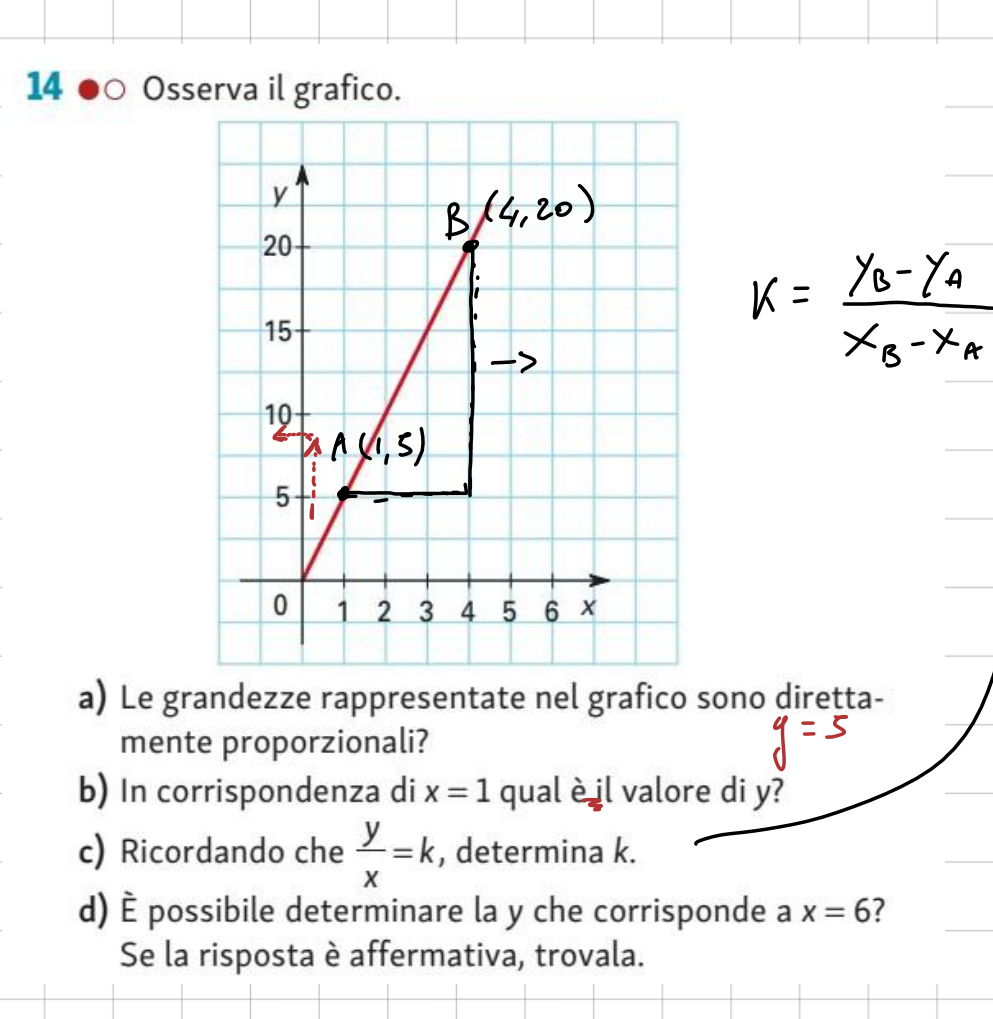
\includegraphics[width=0.78\linewidth]{immagini/traccia_es_14.png}
\caption{Traccia originale dal libro di testo: Esercizio 14, analisi del grafico cartesiano con punti $A(1, 5)$ e $B(4, 20)$.}
\end{figure}

\begin{metodo}[Risoluzione Completa e Commento Fisico]
\begin{enumerate}[label=\alph*)]
  \item \textbf{Verifica della Proporzionalit\`a Diretta:}\\
  Le grandezze rappresentate sono \textbf{direttamente proporzionali}. La traiettoria cartesiana \`e una semiretta uscente dall'origine degli assi $(0, 0)$.

  \item \textbf{Valore di $y$ per $x = 1$:}\\
  Dall'intersezione con la retta nel punto $A$, per $x = 1$ si ricava direttamente $y = 5$.

  \item \textbf{Determinazione della Costante $k$:}\\
  Ricordando che la definizione analitica della proporzionalit\`a diretta \`e $y / x = k$, calcoliamo il rapporto costante per i punti noti:
  \[
  k = \frac{y_A}{x_A} = \frac{5}{1} = 5, \qquad k = \frac{y_B}{x_B} = \frac{20}{4} = 5
  \]
  La costante di proporzionalit\`a vale $\mathbf{k = 5}$, e l'equazione analitica della retta \`e $y = 5x$.

  \item \textbf{Calcolo del valore di $y$ per $x = 6$:}\\
  S\`i, \`e possibile determinare il valore corrispondente applicando l'equazione della retta:
  \[
  y(6) = 5 \cdot 6 = \mathbf{30}
  \]
\end{enumerate}
\end{metodo}

\section{Esercizio 22: Dipendenza Lineare con Intercetta all'Origine}

\begin{figure}[H]
\centering
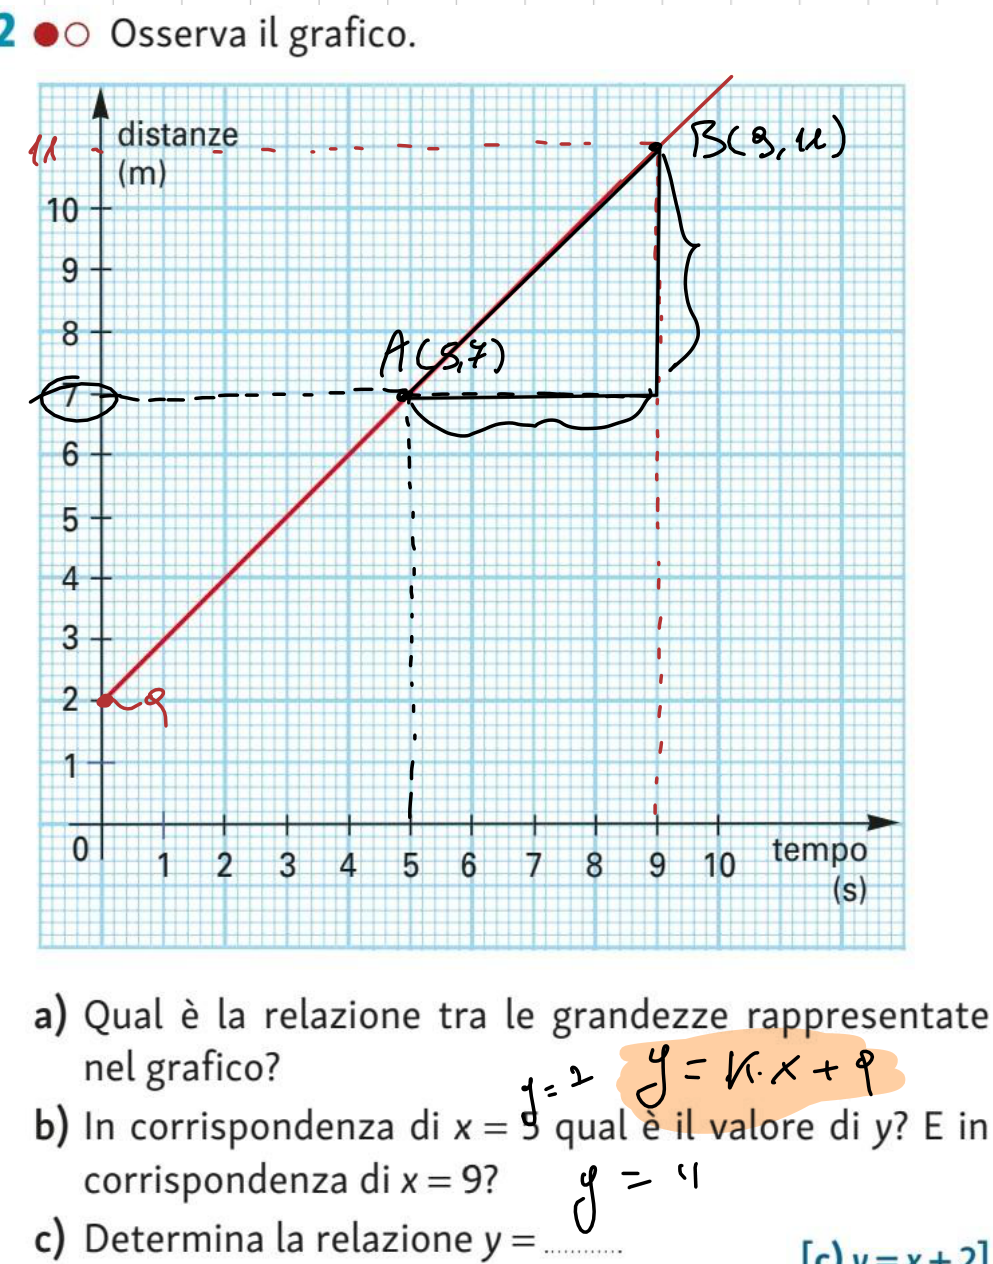
\includegraphics[width=0.78\linewidth]{immagini/traccia_es_22.png}
\caption{Traccia originale dal libro di testo: Esercizio 22, retta non passante per l'origine con punti $A(5, 7)$, $B(9, 11)$ e intercetta $q=2$.}
\end{figure}

\begin{metodo}[Risoluzione Completa e Significato Geometrico]
\begin{enumerate}[label=\alph*)]
  \item \textbf{Relazione tra le Grandezze:}\\
  La relazione \`e una \textbf{dipendenza lineare} del tipo $y = kx + q$ (oppure $y = mx + q$). Non si tratta di una proporzionalit\`a diretta poich\'e la retta non attraversa l'origine $(0, 0)$, bens\`i presenta un'ordinata all'origine non nulla ($q = 2$).

  \item \textbf{Lettura dei Valori dal Grafico:}\\
  Dal grafico si deducono le coordinate dei punti notevoli:
  \begin{itemize}
    \item Per $x = 0$, $y = 2$ (termine noto $q$);
    \item Per $x = 5$, $y = 7$ (punto $A$);
    \item Per $x = 9$, $y = 11$ (punto $B$).
  \end{itemize}

  \item \textbf{Determinazione dell'Equazione Analitica:}\\
  Calcoliamo la pendenza $k$ tramite il rapporto incrementale:
  \[
  k = \frac{\Delta y}{\Delta x} = \frac{y_B - y_A}{x_B - x_A} = \frac{11 - 7}{9 - 5} = \frac{4}{4} = 1
  \]
  Poich\'e per $x = 0$ la retta interseca l'asse delle ordinate a quota $q = 2$, l'equazione completa \`e:
  \[
  \mathbf{\boxed{y = x + 2}}
  \]
\end{enumerate}
\end{metodo}

\section{Esercizio 26: Proporzionalit\`a Inversa e Ramo di Iperbole Equilatera}

\begin{figure}[H]
\centering
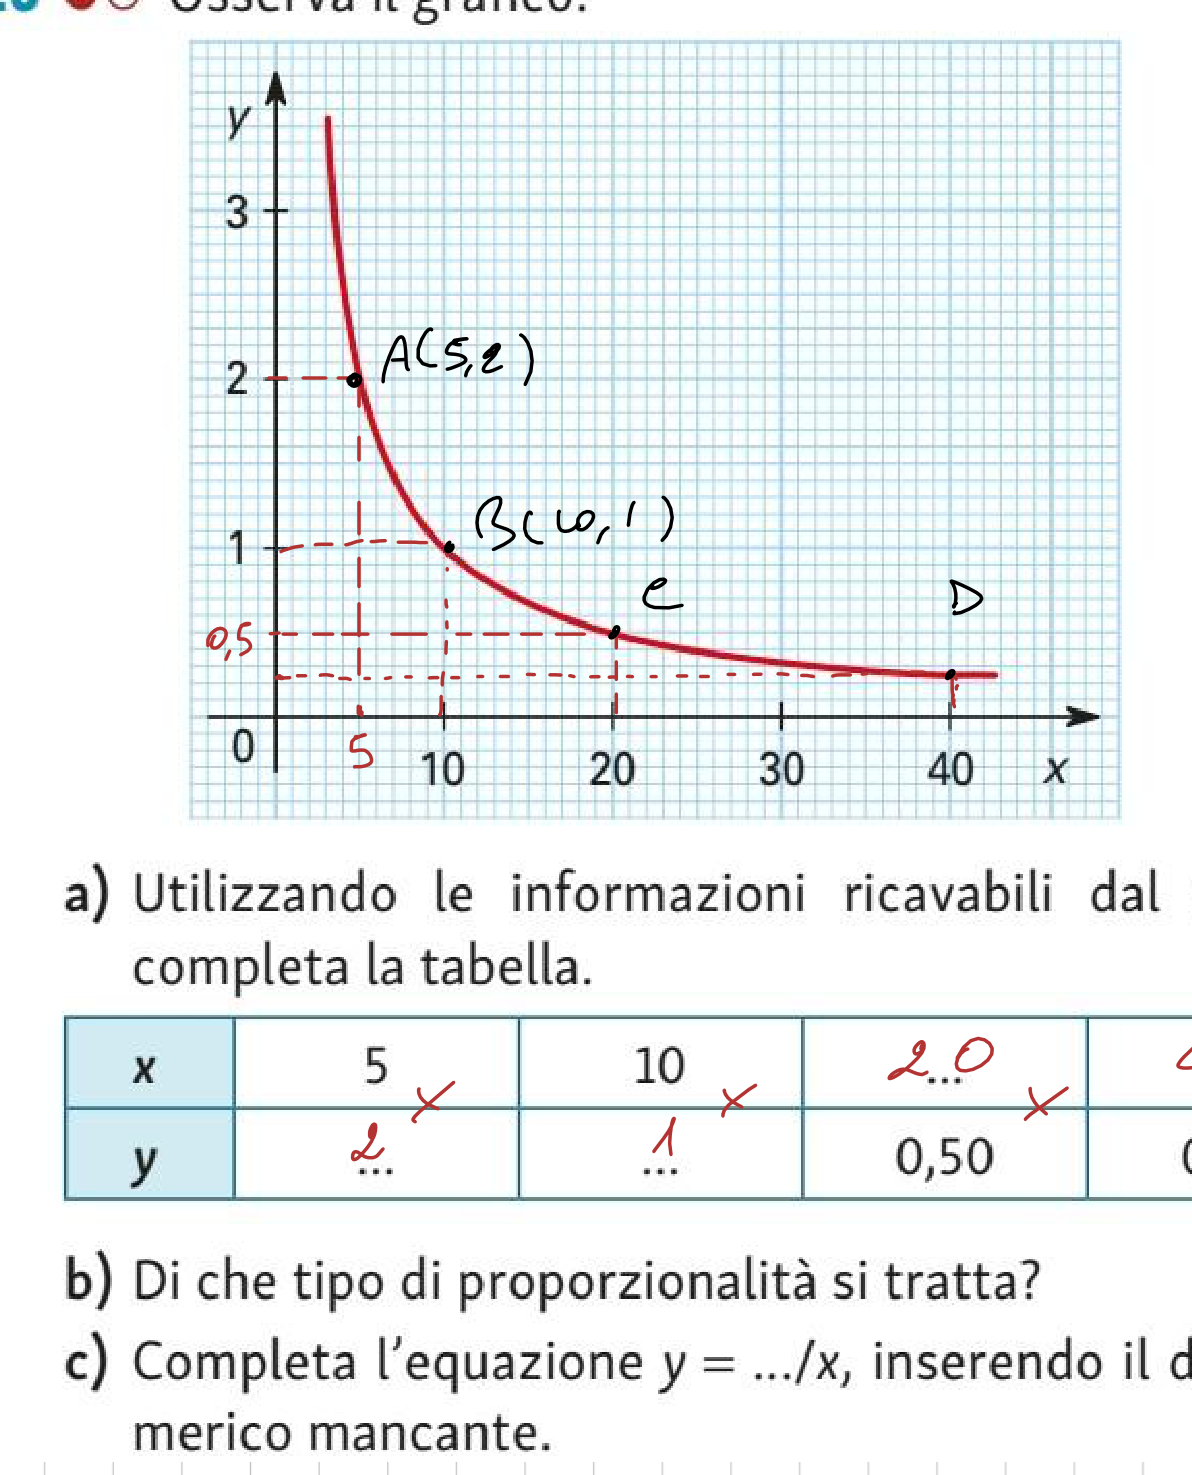
\includegraphics[width=0.78\linewidth]{immagini/traccia_es_26.png}
\caption{Traccia originale dal libro di testo: Esercizio 26, grafico di proporzionalit\`a inversa con punti $A, B, C, D$.}
\end{figure}

\begin{metodo}[Risoluzione Completa e Tabulazione]
\begin{enumerate}[label=\alph*)]
  \item \textbf{Completamento della Tabella dei Valori:}\\
  Leggendo le coordinate dei quattro punti evidenziati sulla curva:
  \begin{itemize}
    \item Punto $A$: per $x = 5$, $y = 2$;
    \item Punto $B$: per $x = 10$, $y = 1$;
    \item Punto $C$: per $x = 20$, $y = 0{,}50$;
    \item Punto $D$: per $x = 40$, $y = 0{,}25$.
  \end{itemize}
  \begin{center}
  \begin{tabular}{ccccc}
  \toprule
  $\mathbf{x}$ & $5$ & $10$ & $20$ & $40$ \\
  $\mathbf{y}$ & $2$ & $1$ & $0{,}50$ & $0{,}25$ \\
  $\mathbf{x \cdot y}$ & $10$ & $10$ & $10$ & $10$ \\
  \bottomrule
  \end{tabular}
  \end{center}

  \item \textbf{Natura della Proporzionalit\`a:}\\
  Poich\'e il prodotto tra le due grandezze si mantiene rigorosamente costante ($x \cdot y = 10$), si tratta di una \textbf{proporzionalit\`a inversa}. La curva geometrica \`e un \textbf{ramo di iperbole equilatera} riferita ai propri asintoti.

  \item \textbf{Equazione Analitica:}\\
  Esplicitando la variabile dipendente $y$:
  \[
  \mathbf{\boxed{y = \frac{10}{x}}}
  \]
\end{enumerate}
\end{metodo}

\begin{figure}[H]
\centering
\begin{tikzpicture}[scale=0.95, >=stealth]
  % Griglia millimetrata soft
  \draw[step=1cm, gray!15, very thin] (0, 0) grid (9.2, 5.5);

  % Assi cartesiani
  \draw[->, thick, primaryBlue] (-0.3, 0) -- (9.5, 0) node[right, font=\small] {$x$};
  \draw[->, thick, primaryBlue] (0, -0.3) -- (0, 5.8) node[above, font=\small] {$y$};
  \node[below left, primaryBlue] at (0, 0) {$O$};

  % Asintoti cartesiani
  \node[above right, font=\scriptsize, gray!60!black] at (0, 5.4) {Asintoto verticale: asse $y$ ($x = 0$)};
  \node[below left, font=\scriptsize, gray!60!black] at (9.4, 0) {Asintoto orizzontale: asse $x$ ($y = 0$)};

  % Curva: ramo di iperbole equilatera y = 10 / x
  % Scala: X_cm = x * 0.2, Y_cm = y * 2.0
  \draw[very thick, accentRed!90!black, domain=3.8:44, samples=80] 
    plot ({\x * 0.2}, {20 / \x});

  % Tratteggi di proiezione e punti sperimentali
  % Punto A (5, 2) -> (1.0, 4.0)
  \draw[dashed, primaryBlue!70] (1.0, 0) -- (1.0, 4.0) -- (0, 4.0);
  \fill[accentRed!90!black] (1.0, 4.0) circle (2.5pt);
  \node[above right, font=\footnotesize\bfseries] at (1.0, 4.0) {$A(5;\, 2)$};
  \node[below, font=\scriptsize] at (1.0, 0) {$5$};
  \node[left, font=\scriptsize] at (0, 4.0) {$2$};

  % Punto B (10, 1) -> (2.0, 2.0)
  \draw[dashed, primaryBlue!70] (2.0, 0) -- (2.0, 2.0) -- (0, 2.0);
  \fill[accentRed!90!black] (2.0, 2.0) circle (2.5pt);
  \node[above right, font=\footnotesize\bfseries] at (2.0, 2.0) {$B(10;\, 1)$};
  \node[below, font=\scriptsize] at (2.0, 0) {$10$};
  \node[left, font=\scriptsize] at (0, 2.0) {$1$};

  % Punto C (20, 0.5) -> (4.0, 1.0)
  \draw[dashed, primaryBlue!70] (4.0, 0) -- (4.0, 1.0) -- (0, 1.0);
  \fill[accentRed!90!black] (4.0, 1.0) circle (2.5pt);
  \node[above right, font=\footnotesize\bfseries] at (4.0, 1.0) {$C(20;\, 0{,}5)$};
  \node[below, font=\scriptsize] at (4.0, 0) {$20$};
  \node[left, font=\scriptsize] at (0, 1.0) {$0{,}5$};

  % Punto D (40, 0.25) -> (8.0, 0.5)
  \draw[dashed, primaryBlue!70] (8.0, 0) -- (8.0, 0.5) -- (0, 0.5);
  \fill[accentRed!90!black] (8.0, 0.5) circle (2.5pt);
  \node[above right, font=\footnotesize\bfseries] at (8.0, 0.5) {$D(40;\, 0{,}25)$};
  \node[below, font=\scriptsize] at (8.0, 0) {$40$};
  \node[left, font=\scriptsize] at (0, 0.5) {$0{,}25$};

  % Didascalia analitica sulla curva
  \node[font=\footnotesize\bfseries, accentRed!90!black, fill=white, fill opacity=0.85, text opacity=1, inner sep=2pt] 
    at (5.5, 3.2) {Ramo di Iperbole Equilatera: $y = \dfrac{10}{x} \iff x \cdot y = 10$};
\end{tikzpicture}
\caption{Grafico cartesiano analitico dell'Esercizio 26: ramo di iperbole equilatera riferita ai propri asintoti cartesiani ($x = 0$ e $y = 0$). Tutti i punti $A, B, C, D$ appartengono alla curva con costante di proporzionalit\`a $k = x \cdot y = 10$.}
\label{fig:iperbole_es26}
\end{figure}

\section{Esercizio 32: Proporzionalit\`a Quadratica e Moto di Caduta di un Sasso}

\begin{figure}[H]
\centering
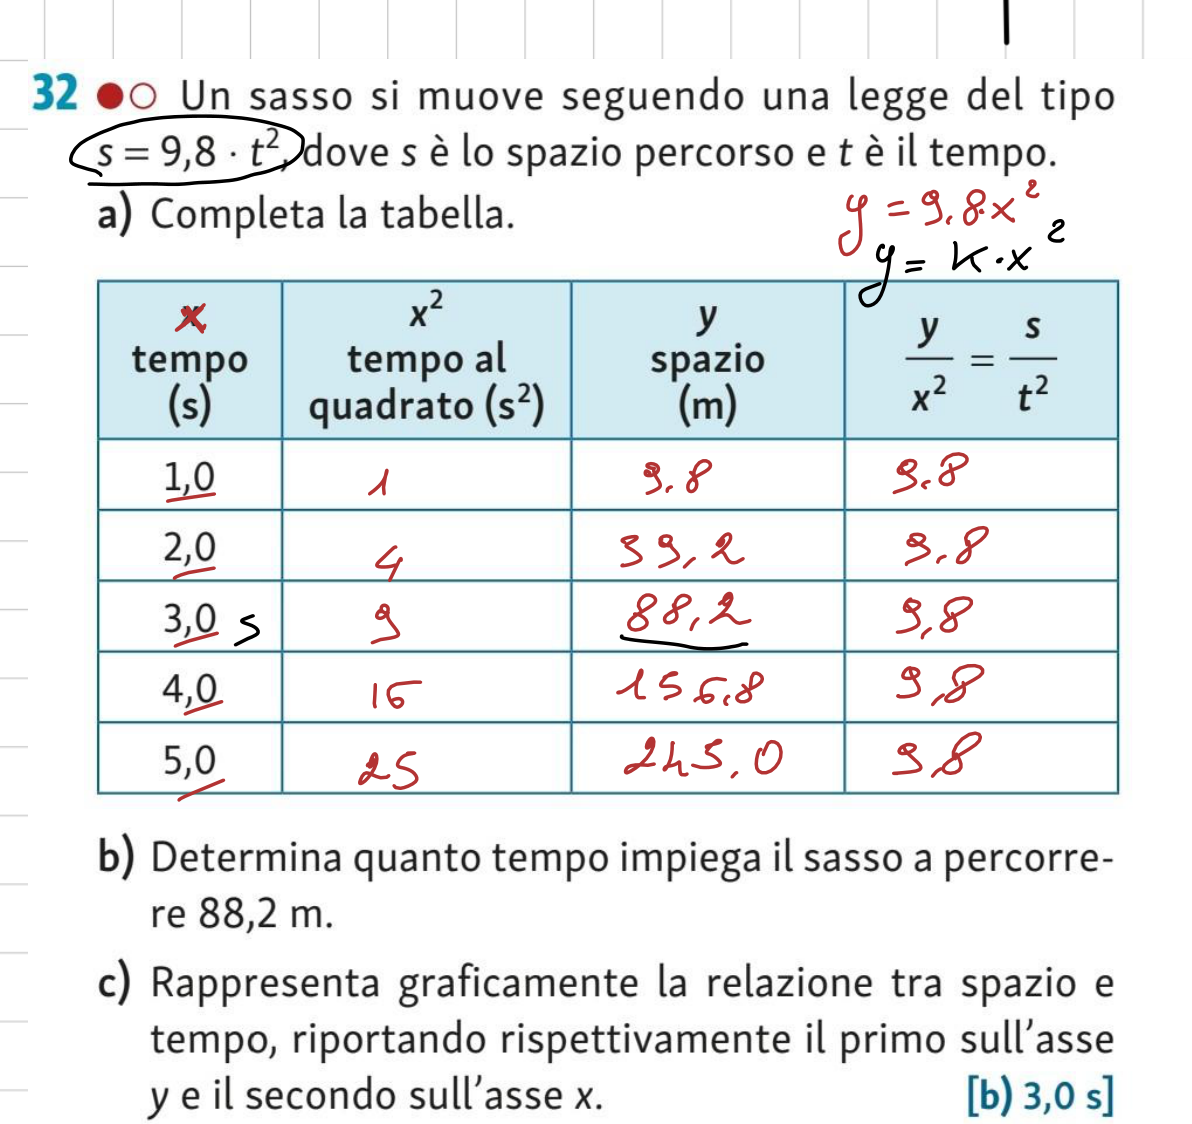
\includegraphics[width=0.78\linewidth]{immagini/traccia_es_32.png}
\caption{Traccia originale dal libro di testo: Esercizio 32, legge oraria quadratica $s = 9{,}8 \cdot t^2$.}
\end{figure}

\begin{metodo}[Risoluzione Completa e Analisi Cinematica]
La legge del moto assegnata \`e $s = 9{,}8 \cdot t^2$, corrispondente al modello di proporzionalit\`a quadratica $y = k x^2$ con costante $k = 9{,}8\,\text{m/s}^2$.
\begin{enumerate}[label=\alph*)]
  \item \textbf{Completamento della Tabella:}\\
  Calcoliamo i quadrati dei tempi e i corrispondenti spazi percorsi:
  \begin{center}
  \begin{tabular}{cccc}
  \toprule
  $\mathbf{x}$ (tempo $t$ in s) & $\mathbf{x^2}$ ($t^2$ in s$^2$) & $\mathbf{y}$ (spazio $s$ in m) & $\mathbf{y / x^2 = s / t^2}$ ($\text{m/s}^2$) \\
  \midrule
  $1{,}0$ & $1$  & $9{,}8$   & $9{,}8$ \\
  $2{,}0$ & $4$  & $39{,}2$  & $9{,}8$ \\
  $3{,}0$ & $9$  & $88{,}2$  & $9{,}8$ \\
  $4{,}0$ & $16$ & $156{,}8$ & $9{,}8$ \\
  $5{,}0$ & $25$ & $245{,}0$ & $9{,}8$ \\
  \bottomrule
  \end{tabular}
  \end{center}

  \item \textbf{Tempo per Percorrere $88{,}2\,\text{m}$:}\\
  Impostiamo l'equazione $s(t) = 88{,}2\,\text{m}$ e ricaviamo $t$ invertendo la relazione quadratica:
  \[
  9{,}8 \cdot t^2 = 88{,}2 \implies t^2 = \frac{88{,}2}{9{,}8} = 9 \implies \mathbf{t = \sqrt{9} = 3{,}0\,\text{s}}
  \]

  \item \textbf{Rappresentazione Grafica:}\\
  Riportando il tempo $t$ sull'asse delle ascisse e lo spazio $s$ sull'asse delle ordinate, la curva ottenuta \`e un \textbf{ramo di parabola} convessa con vertice nell'origine degli assi $(0, 0)$.
\end{enumerate}
\end{metodo}

\section{Esercizio 34: Caduta di un Vaso di Fiori da un Balcone}

\begin{figure}[H]
\centering
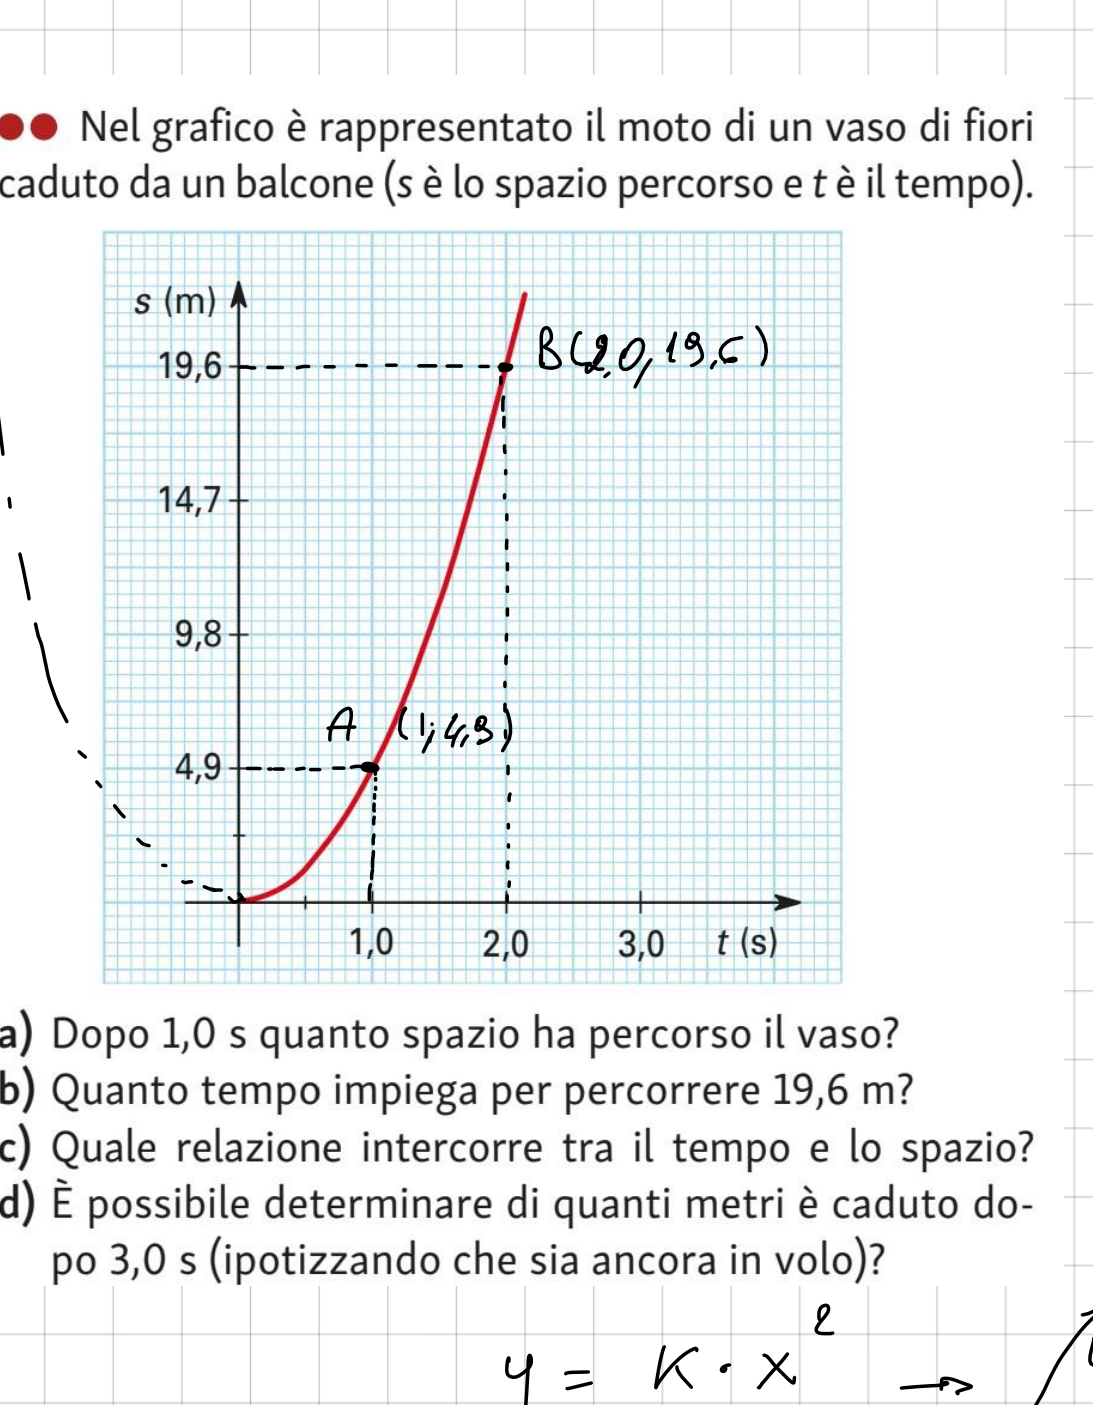
\includegraphics[width=0.78\linewidth]{immagini/traccia_es_34.png}
\caption{Traccia originale dal libro di testo: Esercizio 34, moto di caduta libera di un vaso con punti $A(1{,}0; 4{,}9)$ e $B(2{,}0; 19{,}6)$.}
\end{figure}

\begin{metodo}[Risoluzione Completa e Modello di Caduta Libera]
\begin{enumerate}[label=\alph*)]
  \item \textbf{Spazio percorso dopo $1{,}0\,\text{s}$:}\\
  Dal grafico, in corrispondenza del punto $A(1{,}0; 4{,}9)$ sull'asse delle ascisse $t = 1{,}0\,\text{s}$, si legge direttamente:
  \[
  \mathbf{s = 4{,}9\,\text{m}}
  \]

  \item \textbf{Tempo impiegato per percorrere $19{,}6\,\text{m}$:}\\
  In corrispondenza dell'ordinata $s = 19{,}6\,\text{m}$ (punto $B$), la proiezione sull'asse dei tempi fornisce:
  \[
  \mathbf{t = 2{,}0\,\text{s}}
  \]

  \item \textbf{Relazione tra Tempo e Spazio:}\\
  Valutiamo il rapporto tra lo spazio e il quadrato del tempo per i due punti sperimentali:
  \[
  \frac{s_A}{t_A^2} = \frac{4{,}9\,\text{m}}{(1{,}0\,\text{s})^2} = 4{,}9\,\frac{\text{m}}{\text{s}^2}, \qquad \frac{s_B}{t_B^2} = \frac{19{,}6\,\text{m}}{(2{,}0\,\text{s})^2} = \frac{19{,}6}{4} = 4{,}9\,\frac{\text{m}}{\text{s}^2}
  \]
  Il rapporto \`e costante. La relazione \`e una \textbf{proporzionalit\`a quadratica diretta}:
  \[
  \mathbf{\boxed{s(t) = 4{,}9 \cdot t^2}}
  \]
  \textit{Nota teorica:} La costante $4{,}9\,\text{m/s}^2$ coincide esattamente con $\frac{1}{2}g$, dove $g \approx 9{,}8\,\text{m/s}^2$ \`e l'accelerazione di gravit\`a terrestre: $s = \frac{1}{2}gt^2$.

  \item \textbf{Distanza percorsa dopo $3{,}0\,\text{s}$ (se ancora in volo):}\\
  Sostituendo $t = 3{,}0\,\text{s}$ nella legge oraria quadratica:
  \[
  s(3{,}0) = 4{,}9 \cdot (3{,}0)^2 = 4{,}9 \cdot 9 = \mathbf{\boxed{44{,}1\,\text{m}}}
  \]
\end{enumerate}
\end{metodo}

\section{Esercizio 39: Risoluzione Guidata di un'Equazione Lineare}

\begin{figure}[H]
\centering
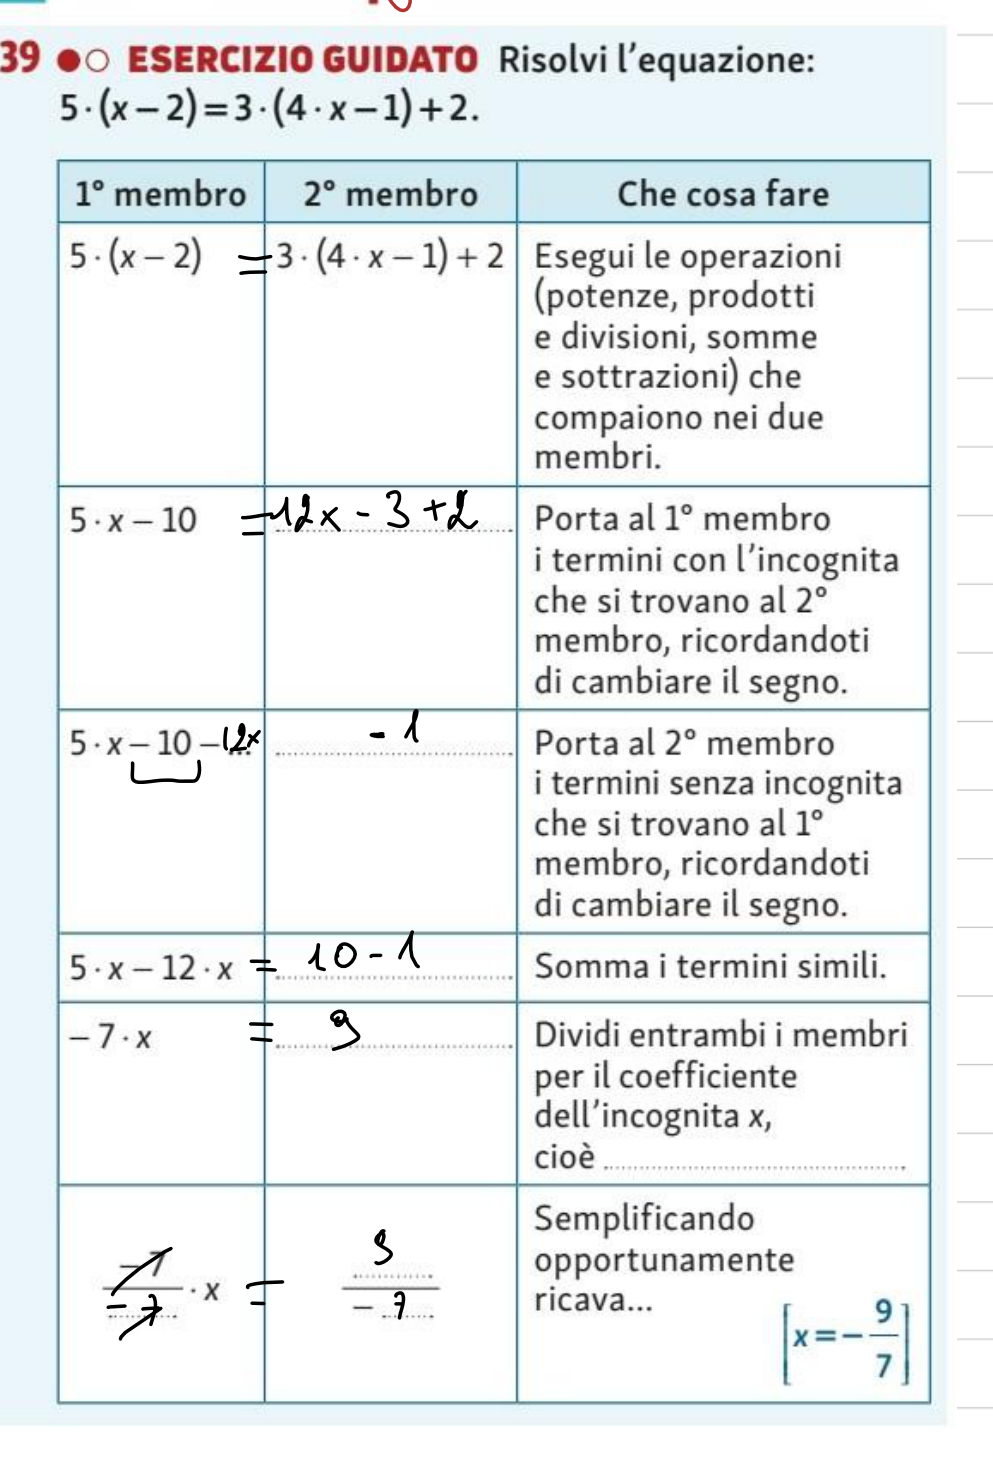
\includegraphics[width=0.78\linewidth]{immagini/traccia_es_39.png}
\caption{Traccia originale dal libro di testo: Esercizio 39, tabella guidata per la risoluzione dell'equazione $5(x-2) = 3(4x-1) + 2$.}
\end{figure}

\begin{metodo}[Applicazione Rigorosa dei Principi di Equivalenza]
Equazione iniziale assegnata:
\[
5(x - 2) = 3(4x - 1) + 2
\]
\begin{enumerate}
  \item \textbf{Esecuzione delle operazioni algebriche nei due membri:}\\
  Sviluppiamo le moltiplicazioni distribuendo i fattori numerici:
  \[
  5x - 10 = 12x - 3 + 2 \implies 5x - 10 = 12x - 1
  \]

  \item \textbf{Applicazione del Primo Principio di Equivalenza (trasporto dell'incognita):}\\
  Sottraiamo $12x$ da ambo i membri (portiamo i termini con l'incognita a sinistra cambiandone il segno):
  \[
  5x - 10 - 12x = -1
  \]

  \item \textbf{Applicazione del Primo Principio di Equivalenza (trasporto dei termini noti):}\\
  Aggiungiamo $10$ ad ambo i membri (portiamo $-10$ a destra come $+10$):
  \[
  5x - 12x = 10 - 1
  \]

  \item \textbf{Somma dei termini simili:}\\
  \[
  -7x = 9
  \]

  \item \textbf{Applicazione del Secondo Principio di Equivalenza (divisione per il coefficiente):}\\
  Dividiamo entrambi i membri per il coefficiente di $x$, ossia per $-7 \neq 0$:
  \[
  \frac{-7x}{-7} = \frac{9}{-7} \implies \mathbf{\boxed{x = -\frac{9}{7}}}
  \]
\end{enumerate}
\end{metodo}

% ==============================================================================
% CAPITOLO: UNITÀ DI MISURA DERIVATE, VOLUME E ANALISI DIMENSIONALE (TAVOLA 14)
% ==============================================================================
\chapter{Unit\`a di Misura Derivate, Volume e Analisi Dimensionale Rigorosa}

\section{La Misura del Volume: Il Litro, Equivalenze Geometriche e Densit\`a dell'Acqua}

\begin{definizione}[Volume e Litro come Unit\`a di Capacit\`a (Tavola 14)]
Nel Sistema Internazionale l'unit\`a di misura del volume \`e il \textbf{metro cubo} ($\mathrm{m}^3$). Per i fluidi e i liquidi si adotta comunemente l'\textbf{unit\`a di capacit\`a}: il \textbf{litro} ($\mathrm{L}$).
L'equivalenza fondamentale che raccorda le unit\`a di volume con la capacit\`a \`e:
\begin{equation}
    \mathbf{1\,\mathrm{dm}^3 = 1\,\mathrm{L}}
\end{equation}
ovvero: un litro corrisponde esattamente allo spazio occupato da un cubo avente il lato di un decimetro ($10\,\mathrm{cm}$).
\end{definizione}

\begin{metodo}[Scala delle Equivalenze: Volumi Cubici e Capacit\`a in Litri]
Poich\'e le unit\`a volumetriche scalano secondo il cubo dei prefissi lineari ($10^3 = 1000$):
\begin{center}
\renewcommand{\arraystretch}{1.3}
\begin{tabular}{ccccccc}
$\mathbf{m^3}$ & $\longleftrightarrow$ & $\mathbf{dm^3}$ & $\longleftrightarrow$ & $\mathbf{cm^3}$ & $\longleftrightarrow$ & $\mathbf{mm^3}$ \\
$\parallel$ & & $\parallel$ & & $\parallel$ & & \\
$\mathrm{kL}$ & $\mathrm{hL}\quad\mathrm{daL}$ & $\mathbf{L}$ & $\mathrm{dL}\quad\mathrm{cL}$ & $\mathbf{mL}$ & & \\
\end{tabular}
\end{center}
In particolare:
\begin{itemize}[leftmargin=2em]
    \item $1\,\mathrm{m}^3 = 1000\,\mathrm{dm}^3 = 1000\,\mathrm{L} = 1\,\mathrm{kL}$ (un metro cubo equivale a mille litri).
    \item $1\,\mathrm{dm}^3 = 1\,\mathrm{L} = 1000\,\mathrm{mL} = 1000\,\mathrm{cm}^3 \implies \mathbf{1\,\mathrm{cm}^3 = 1\,\mathrm{mL}}$.
\end{itemize}
\end{metodo}

\begin{commento}[La Densit\`a dell'Acqua Distillata e la Coerenza delle Unit\`a di Misura]
La densit\`a dell'acqua pura a temperatura di $4\,^\circ\mathrm{C}$ \`e convenzionalmente pari a $1000\,\mathrm{kg/m^3}$:
\begin{equation}
    d_{\mathrm{acqua}} = 1000\,\frac{\mathrm{kg}}{\mathrm{m}^3} = \frac{1000\,\mathrm{kg}}{1000\,\mathrm{dm}^3} = 1\,\frac{\mathrm{kg}}{\mathrm{dm}^3} = \mathbf{1\,\frac{\mathrm{kg}}{\mathrm{L}}}
\end{equation}
Un litro d'acqua pura possiede esattamente la massa di un chilogrammo!
\end{commento}

\section{Il Metodo dell'Analisi Dimensionale e Verifica di Congruenza delle Equazioni}

\begin{definizione}[Analisi Dimensionale di un'Equazione Fisica (Tavola 14)]
L'\textbf{analisi dimensionale} di un'equazione in cui compaiono delle grandezze fisiche consiste nel \textbf{verificare la congruenza delle unit\`a di misura in cui sono espressi i suoi due membri}.\\
\textbf{Regola aurea:} \textit{Le dimensioni fisiche e le unit\`a di misura del primo membro devono essere identiche a quelle del secondo membro.}
\end{definizione}

\begin{metodo}[Verifica Comparativa della Formula del Volume: $V = m \cdot d$ vs $V = \frac{m}{d}$]
Siano date la massa $m$ ($[M] = \mathrm{kg}$) e la densit\`a $d = \frac{m}{V}$ $\left(\left[\frac{M}{L^3}\right] = \frac{\mathrm{kg}}{\mathrm{m}^3}\right)$. Vogliamo ricavare la formula per il volume $V$ ($[L^3] = \mathrm{m}^3$).

\begin{enumerate}[leftmargin=2em]
    \item \textbf{Test dell'ipotesi errata $V = m \cdot d$:}
    \begin{align}
        1^\circ\text{ Membro: } & [V] = [\mathrm{m}^3] = [L^3] \\
        2^\circ\text{ Membro: } & [m \cdot d] = [\mathrm{kg}] \cdot \left[\frac{\mathrm{kg}}{\mathrm{m}^3}\right] = \left[M \cdot \frac{M}{L^3}\right] = \left[\frac{M^2}{L^3}\right] = \left[\frac{\mathrm{kg}^2}{\mathrm{m}^3}\right]
    \end{align}
    Poich\'e $[L^3] \neq \left[\frac{M^2}{L^3}\right]$, l'uguaglianza \`e \textbf{dimensionalmente falsa} ($\text{\textcolor{accentRed}{\textbf{ERRORE!}}}$). Moltiplicare la massa per la densit\`a non produce un volume!
    
    \item \textbf{Test della formula corretta $V = \frac{m}{d}$:}
    \begin{align}
        1^\circ\text{ Membro: } & [V] = [\mathrm{m}^3] = [L^3] \\
        2^\circ\text{ Membro: } & \left[\frac{m}{d}\right] = \left[\frac{\mathrm{kg}}{\frac{\mathrm{kg}}{\mathrm{m}^3}}\right] = \left[\frac{\mathrm{kg}}{1} \cdot \frac{\mathrm{m}^3}{\mathrm{kg}}\right] = [\mathrm{m}^3] = [L^3]
    \end{align}
    Poich\'e $[L^3] = [L^3]$, la congruenza dimensionale \`e \textbf{perfettamente verificata} ($\text{\textcolor{accentGreen}{\textbf{CORRETTO!}}}$).
\end{enumerate}
\end{metodo}

\begin{figure}[htbp]
\centering
\begin{tikzpicture}[scale=1.1]
    \draw[line width=1.2pt, accentRed, fill=accentRed!5!white, rounded corners=6pt] (-5.5, -2) rectangle (-0.5, 2);
    \node at (-3, 1.5) [font=\bfseries\sffamily, color=accentRed] {Ipotesi Errata: $V = m \cdot d$};
    \node at (-3, 0.7) [font=\small] {$1^\circ$ Membro: $[V] = \mathrm{m}^3 = [L^3]$};
    \node at (-3, 0.0) [font=\small] {$2^\circ$ Membro: $[m \cdot d] = \mathrm{kg} \cdot \frac{\mathrm{kg}}{\mathrm{m}^3} = \frac{\mathrm{kg}^2}{\mathrm{m}^3}$};
    \node at (-3, -0.7) [font=\small\bfseries, color=accentRed] {$[L^3] \neq \left[\frac{M^2}{L^3}\right]$};
    \node at (-3, -1.4) [font=\Large\bfseries, color=accentRed] {\textbf{INCONGRUENTE \texttimes}};

    \draw[line width=1.2pt, accentGreen, fill=accentGreen!5!white, rounded corners=6pt] (0.5, -2) rectangle (5.5, 2);
    \node at (3, 1.5) [font=\bfseries\sffamily, color=accentGreen] {Formula Corretta: $V = \frac{m}{d}$};
    \node at (3, 0.7) [font=\small] {$1^\circ$ Membro: $[V] = \mathrm{m}^3 = [L^3]$};
    \node at (3, 0.0) [font=\small] {$2^\circ$ Membro: $\left[\frac{m}{d}\right] = \frac{\mathrm{kg}}{\mathrm{kg}/\mathrm{m}^3} = \mathrm{m}^3$};
    \node at (3, -0.7) [font=\small\bfseries, color=accentGreen] {$[L^3] = [L^3]$};
    \node at (3, -1.4) [font=\Large\bfseries, color=accentGreen] {\textbf{CONGRUENTE \checkmark}};
\end{tikzpicture}
\caption{Quadro comparativo dell'analisi dimensionale (Tavola 14 del quaderno): verifica della coerenza delle unit\`a di misura tra l'errata moltiplicazione $V = m \cdot d$ e la corretta divisione $V = \frac{m}{d}$.}
\label{fig:analisi_dimensionale_volume}
\end{figure}

% ==============================================================================
% CAPITOLO 9: LA MISURA OPERATIVA, SENSIBILITÀ, INCERTEZZA E MISURE DIRETTE/INDIRETTE (TAVOLE 15-16)
% ==============================================================================
\chapter{La Misura Operativa, Errore di Sensibilit\`a, Incertezza e Misure Dirette vs Indirette}

\section{Misura della Lunghezza di un'Asta con il Righello ed Errore di Sensibilit\`a (Tavola 15)}

Misurare una grandezza fisica significa confrontarla con l'unit\`a di misura campione mediante uno strumento tarato. Consideriamo l'esperimento fondamentale illustrato nella \textbf{Tavola 15} del quaderno: la misura della lunghezza $L$ di un'asta rigida tramite un righello graduato (o un metro da sarti) avente tacche spaziate ogni $0{,}5\,\mathrm{cm}$.

\begin{metodo}[Procedura Operativa di Lettura sulla Scala Graduata]
Per eseguire correttamente la lettura della lunghezza $L$ dell'asta:
\begin{enumerate}[leftmargin=2em]
    \item Si allinea con precisione l'estremit\`a sinistra dell'asta con la tacca dello \textbf{zero} ($0{,}0\,\mathrm{cm}$) della scala graduata, evitando disallineamenti o errori di parallasse.
    \item Si osserva la posizione dell'estremit\`a destra dell'asta rispetto alla scala e \textbf{si considera la tacca pi\`u vicina}: nel nostro caso l'estremit\`a cade sulla tacca intermedia tra $6\,\mathrm{cm}$ e $7\,\mathrm{cm}$, per cui:
    \[
        \mathbf{L = 6{,}5\,\mathrm{cm}}
    \]
    \item Poich\'e nessuna scala graduata pu\`o avere suddivisioni infinitamente fitte, \textbf{tutti gli strumenti di misura sono caratterizzati da un errore di sensibilit\`a}.
\end{enumerate}
\end{metodo}

\begin{figure}[H]
\centering
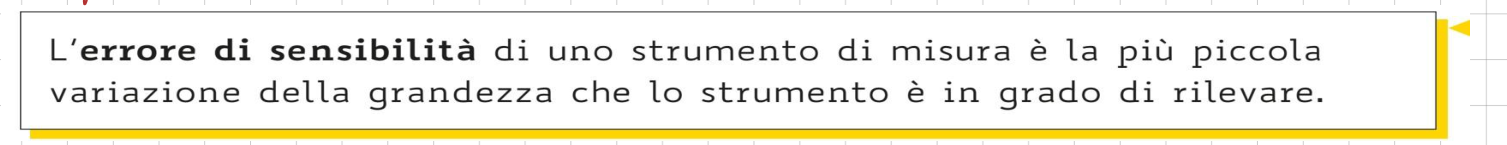
\includegraphics[width=0.82\linewidth]{immagini/traccia_sensibilita_p15.png}
\caption{Definizione dal libro di testo (Tavola 15): l'errore di sensibilit\`a di uno strumento di misura.}
\label{fig:traccia_sensibilita_p15}
\end{figure}

\begin{definizione}[Errore di Sensibilit\`a di uno Strumento di Misura (Tavola 15)]
L'\textbf{errore di sensibilit\`a} (o semplicemente \textbf{sensibilit\`a}) di uno strumento di misura \`e la \textbf{pi\`u piccola variazione della grandezza che lo strumento \`e in grado di rilevare}.\\
Operativamente, su uno strumento analogico a scala graduata, l'errore di sensibilit\`a \`e la \textbf{``distanza'' (differenza di valore) tra una tacca e quella immediatamente successiva}.
Nel caso del metro da sarti (o righello graduato al mezzo centimetro) rappresentato nella Tavola 15, prendendo due tacche consecutive qualsiasi (ad esempio $7{,}5\,\mathrm{cm}$ e $8{,}0\,\mathrm{cm}$), la sensibilit\`a vale:
\begin{equation}
    \mathbf{\Delta x = 8{,}0\,\mathrm{cm} - 7{,}5\,\mathrm{cm} = 0{,}5\,\mathrm{cm}}
\end{equation}
\end{definizione}

\begin{figure}[htbp]
\centering
\begin{tikzpicture}[scale=1.15, >=stealth]
    % Corpo del righello graduato (da 0 a 8 cm)
    \fill[primaryBlue!4!white, draw=primaryBlue!80!black, line width=1.2pt, rounded corners=2pt]
        (-0.4, 1.0) rectangle (8.8, 2.3);

    % Tacche del righello (passo 0.5 cm da 0.0 a 8.0)
    \foreach \x in {0, 1, ..., 8} {
        \draw[line width=1.3pt, primaryBlue!90!black] (\x, 2.3) -- (\x, 1.75);
        \node[font=\small\bfseries, color=primaryBlue!90!black, fill=white, fill opacity=0.9, text opacity=1, inner sep=1pt]
            at (\x, 1.42) {$\x$};
    }
    \foreach \x in {0.5, 1.5, ..., 7.5} {
        \draw[line width=0.9pt, primaryBlue!80!black] (\x, 2.3) -- (\x, 1.92);
    }
    \node[font=\footnotesize\bfseries, color=primaryBlue!80!black] at (8.45, 1.42) {$\mathrm{cm}$};

    % Linee di proiezione tratteggiate rosse (da 0.0 cm e da 6.5 cm)
    \draw[dashed, line width=1.2pt, accentRed] (0.0, 2.45) -- (0.0, 0.15);
    \draw[dashed, line width=1.2pt, accentRed] (6.5, 2.45) -- (6.5, 0.15);

    % Asta rossa sotto il righello (da 0.0 a 6.5 cm)
    \fill[accentRed!85!white, draw=accentRed!90!black, line width=1.2pt, rounded corners=1.5pt]
        (0.0, 0.35) rectangle (6.5, 0.65);
    \node[font=\small\bfseries, color=accentRed!90!black, fill=white, fill opacity=0.9, text opacity=1, inner sep=2pt]
        at (3.25, -0.05) {Lunghezza dell'asta (tacca pi\`u vicina): $L = 6{,}5\,\mathrm{cm}$};

    % Evidenziazione della sensibilita tra 7.5 cm e 8.0 cm con frecce rosse
    \draw[->, line width=1.4pt, accentRed] (7.5, 3.05) -- (7.5, 2.35);
    \draw[->, line width=1.4pt, accentRed] (8.0, 3.05) -- (8.0, 2.35);
    \draw[<->, line width=1.0pt, accentAmber!90!black] (7.5, 2.75) -- (8.0, 2.75);

    \node[font=\footnotesize\bfseries, color=accentRed!90!black, fill=white, fill opacity=0.9, text opacity=1, inner sep=2pt]
        at (6.2, 3.38) {Distanza tra due tacche consecutive: $\Delta x = 8{,}0 - 7{,}5 = 0{,}5\,\mathrm{cm}$};

    % Etichetta allineamento zero
    \node[font=\footnotesize\bfseries, color=primaryBlue, fill=white, fill opacity=0.9, text opacity=1, inner sep=1.5pt]
        at (1.25, 2.75) {Allineamento a $0{,}0\,\mathrm{cm}$};
    \draw[->, thick, primaryBlue] (0.45, 2.75) -- (0.05, 2.40);
\end{tikzpicture}
\caption{Rappresentazione vettoriale della misura diretta della lunghezza di un'asta con il righello graduato (Tavola 15): l'estremit\`a destra cade in corrispondenza della tacca $6{,}5\,\mathrm{cm}$, mentre la distanza tra due tacche consecutive ($7{,}5\,\mathrm{cm}$ e $8{,}0\,\mathrm{cm}$) definisce l'errore di sensibilit\`a $\Delta x = 0{,}5\,\mathrm{cm}$.}
\label{fig:misura_righello_tav15}
\end{figure}

\section{L'Incertezza $\Delta x$ e la Scrittura Formale di una Misura (Tavola 15)}

\begin{figure}[H]
\centering
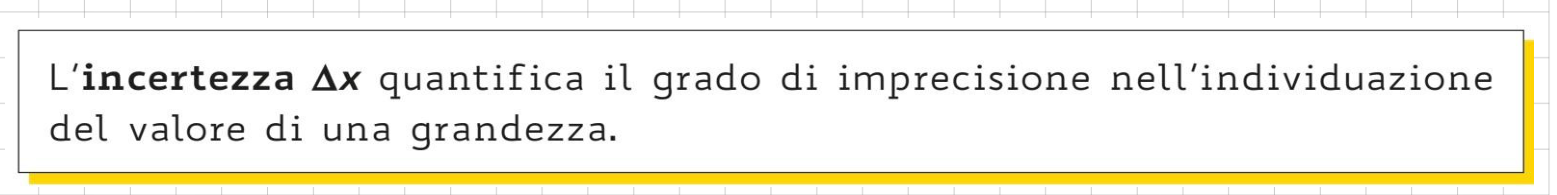
\includegraphics[width=0.82\linewidth]{immagini/traccia_incertezza_p15.png}
\caption{Definizione dal libro di testo (Tavola 15): l'incertezza $\Delta x$ di una misura.}
\label{fig:traccia_incertezza_p15}
\end{figure}

\begin{definizione}[Incertezza $\Delta x$ e Scrittura Formale della Misura (Tavola 15)]
L'\textbf{incertezza $\Delta x$} quantifica il \textbf{grado di imprecisione nell'individuazione del valore di una grandezza}.\\
\textbf{Regola fondamentale per la misura singola:} \textit{Se misuriamo una sola volta la lunghezza di un'asta con il righello, l'\textbf{incertezza} e la \textbf{sensibilit\`a} dello strumento sono sinonimi} ($\Delta x = \text{sensibilit\`a}$).

La misura completa di una grandezza fisica $X$ si scrive sempre nella forma canonica:
\begin{equation}
    \mathbf{\boxed{X = (x_m \pm \Delta x)\,\mathrm{udm}}}
\end{equation}
dove:
\begin{itemize}[leftmargin=2em]
    \item $\mathbf{X}$ \`e il \textbf{simbolo della grandezza fisica} misurata (es. $L$ per una lunghezza, $m$ per una massa, $t$ per un tempo);
    \item $\mathbf{x_m}$ \`e il \textbf{valore della grandezza} (il valore misurato letto sulla tacca pi\`u vicina, o il valore medio in caso di misure ripetute);
    \item $\mathbf{\Delta x}$ \`e l'\textbf{incertezza assoluta} associata alla misura;
    \item $\mathbf{\mathrm{udm}}$ \`e l'\textbf{unit\`a di misura}, posta fuori dalle parentesi tonde poich\'e si riferisce sia a $x_m$ sia a $\Delta x$.
\end{itemize}
\end{definizione}

\begin{figure}[htbp]
\centering
\begin{tikzpicture}[scale=1.05, >=stealth]
    % Riquadro centrale formula
    \draw[line width=1.4pt, primaryBlue, fill=primaryBlue!5!white, rounded corners=6pt]
        (-4.2, -0.75) rectangle (4.2, 0.75);

    \node[font=\LARGE\bfseries, color=primaryBlue!95!black] at (0, 0)
        {$X \;=\; (\,x_m \;\pm\; \Delta x\,)\;\mathrm{udm}$};

    % Frecce e legende esplicative (stile Tavola 15)
    % X -> simbolo della grandezza
    \draw[->, line width=1.2pt, accentRed] (-2.55, -0.45) -- (-3.4, -1.45);
    \node[font=\small\bfseries, color=accentRed, fill=white, fill opacity=0.9, text opacity=1, inner sep=2pt]
        at (-3.6, -1.75) {Simbolo della grandezza ($X$)};

    % x_m -> valore della grandezza
    \draw[->, line width=1.2pt, primaryBlue] (-0.75, 0.50) -- (-1.6, 1.45);
    \node[font=\small\bfseries, color=primaryBlue, fill=white, fill opacity=0.9, text opacity=1, inner sep=2pt]
        at (-1.8, 1.75) {Valore della grandezza ($x_m$)};

    % Delta x -> incertezza / sensibilita
    \draw[->, line width=1.2pt, accentAmber!90!black] (0.85, 0.50) -- (1.8, 1.45);
    \node[font=\small\bfseries, color=accentAmber!90!black, fill=white, fill opacity=0.9, text opacity=1, inner sep=2pt]
        at (2.2, 1.75) {Incertezza / Sensibilit\`a ($\Delta x$)};

    % udm -> unita di misura
    \draw[->, line width=1.2pt, accentGreen!85!black] (2.45, -0.45) -- (3.3, -1.45);
    \node[font=\small\bfseries, color=accentGreen!85!black, fill=white, fill opacity=0.9, text opacity=1, inner sep=2pt]
        at (3.4, -1.75) {Unit\`a di misura ($\mathrm{udm}$)};
\end{tikzpicture}
\caption{Anatomia della scrittura formale di una misura fisica secondo lo schema della Tavola 15.}
\label{fig:anatomia_scrittura_misura}
\end{figure}

\begin{metodo}[Applicazione all'Asta della Tavola 15 e Significato Fisico dell'Intervallo]
Sostituendo i valori rilevati per l'asta ($x_m = 6{,}5\,\mathrm{cm}$ e $\Delta x = 0{,}5\,\mathrm{cm}$), la misura va scritta formalmente come:
\begin{equation}
    \mathbf{\boxed{L = (6{,}5 \pm 0{,}5)\,\mathrm{cm}}}
\end{equation}
\begin{itemize}[leftmargin=2em]
    \item \textbf{Intervallo di incertezza (o di confidenza):} Scrivere $L = (6{,}5 \pm 0{,}5)\,\mathrm{cm}$ significa affermare che la lunghezza reale dell'asta \`e compresa tra un valore minimo $L_{\min}$ e un valore massimo $L_{\max}$:
    \[
        L_{\min} = 6{,}5 - 0{,}5 = 6{,}0\,\mathrm{cm}, \quad L_{\max} = 6{,}5 + 0{,}5 = 7{,}0\,\mathrm{cm} \implies L \in [6{,}0;\; 7{,}0]\,\mathrm{cm}
    \]
    \item \textbf{Coerenza delle cifre decimali:} L'incertezza $\Delta x = 0{,}5\,\mathrm{cm}$ \`e espressa con una sola cifra significativa (sulla posizione dei decimi di centimetro), e il valore misurato $x_m = 6{,}5\,\mathrm{cm}$ \`e arrotondato esattamente alla medesima posizione decimale (i decimi).
    \item \textbf{Precisione della misura (Errore Relativo e Percentuale):}
    \[
        e_r = \frac{\Delta L}{L_m} = \frac{0{,}5\,\mathrm{cm}}{6{,}5\,\mathrm{cm}} = \frac{1}{13} \approx 0{,}0769 \quad \implies \quad e_p = e_r \cdot 100\% \approx \mathbf{7{,}7\%}
    \]
\end{itemize}
\end{metodo}

\section{Misure Dirette e Misure Indirette (Tavole 15 e 16)}

Le procedure sperimentali con cui si determina il valore di una grandezza fisica si suddividono in due categorie fondamentali: \textbf{misure dirette} e \textbf{misure indirette}.

\begin{definizione}[Misura Diretta vs Misura Indiretta (Tavole 15 e 16)]
\begin{enumerate}[leftmargin=2em]
    \item \textbf{Misura Diretta (Tavola 15):}\\
    Una misura si dice \textbf{diretta} se il valore della grandezza fisica viene \textbf{letto direttamente dal display} (negli strumenti digitali) \textbf{o dalla scala graduata} (negli strumenti analogici) dello strumento di misura, confrontando direttamente la grandezza con l'unit\`a campione.\\
    \textit{Esempi:} la misura della lunghezza $L = (6{,}5 \pm 0{,}5)\,\mathrm{cm}$ di un'asta con il righello; la lettura della massa su una bilancia; la lettura di un intervallo di tempo con un cronometro o della temperatura con un termometro.

    \item \textbf{Misura Indiretta (Tavola 16):}\\
    Una misura si dice \textbf{indiretta} se il valore della grandezza viene ottenuto \textbf{mediante calcoli algebrici} (applicando una formula matematica o geometrica) a partire dai valori di altre grandezze misurate direttamente.\\
    \textit{Esempio canonico (Tavola 16):} la misura della \textbf{superficie del pavimento} di una stanza ($S = a \cdot b$), determinata moltiplicando tra loro le lunghezze dei due lati $a$ e $b$ misurate direttamente con il metro.
\end{enumerate}
\end{definizione}

\begin{metodo}[Esempio Svolto Completo: Misura Indiretta della Superficie di un Pavimento (Tavola 16)]
Vogliamo determinare la superficie $S$ di un pavimento rettangolare.
\begin{enumerate}[leftmargin=2em]
    \item \textbf{Fase 1 — Misure Dirette dei Lati:} Con una rotella metrica (sensibilit\`a $\Delta x = 0{,}1\,\mathrm{m}$) misuriamo direttamente la lunghezza $a$ e la larghezza $b$ della stanza:
    \[
        a = (4{,}0 \pm 0{,}1)\,\mathrm{m}, \qquad b = (3{,}0 \pm 0{,}1)\,\mathrm{m}
    \]
    \item \textbf{Fase 2 — Calcolo Algebrico del Valore Attendibile (Misura Indiretta):} Applichiamo la formula geometrica dell'area del rettangolo:
    \[
        S_m = a_m \cdot b_m = 4{,}0\,\mathrm{m} \cdot 3{,}0\,\mathrm{m} = \mathbf{12{,}0\,\mathrm{m}^2}
    \]
    \item \textbf{Fase 3 — Propagazione dell'Incertezza sul Prodotto:} Poich\'e la superficie \`e il prodotto di due grandezze affette da incertezza, l'errore relativo sul prodotto \`e la somma degli errori relativi sui singoli fattori:
    \[
        e_{r,S} = \frac{\Delta a}{a_m} + \frac{\Delta b}{b_m} = \frac{0{,}1}{4{,}0} + \frac{0{,}1}{3{,}0} = 0{,}025 + 0{,}0333 = 0{,}0583
    \]
    Da cui l'incertezza assoluta $\Delta S$ sulla superficie vale:
    \[
        \Delta S = S_m \cdot e_{r,S} = 12{,}0\,\mathrm{m}^2 \cdot 0{,}0583 = 0{,}7\,\mathrm{m}^2
    \]
    \item \textbf{Scrittura Formale della Misura Indiretta:}
    \[
        \mathbf{\boxed{S = (12{,}0 \pm 0{,}7)\,\mathrm{m}^2}}
    \]
\end{enumerate}
\end{metodo}

\begin{table}[htbp]
\centering
\small
\renewcommand{\arraystretch}{1.35}
\begin{tabularx}{\textwidth}{lXX}
\toprule
\textbf{Caratteristica} & \textbf{Misura Diretta (Tavola 15)} & \textbf{Misura Indiretta (Tavola 16)} \\
\midrule
\textbf{Procedura Operativa} & Lettura immediata sulla scala graduata o sul display dello strumento. & Calcolo algebrico tramite una formula matematica a partire da misure dirette. \\
\textbf{Origine dell'Incertezza} & Per singola misura coincide direttamente con l'errore di sensibilit\`a $\Delta x$ dello strumento. & Si ottiene mediante le leggi di propagazione degli errori a partire dalle incertezze delle grandezze dirette. \\
\textbf{Esempi di Laboratorio} & Lunghezza dell'asta col righello $L = (6{,}5 \pm 0{,}5)\,\mathrm{cm}$; tempo col cronometro; massa con la bilancia. & Superficie del pavimento $S = a \cdot b$; volume di un cilindro $V = \pi r^2 h$; densit\`a $d = m/V$; velocit\`a $v = s/t$. \\
\bottomrule
\end{tabularx}
\caption{Quadro sinottico comparativo tra misure dirette e misure indirette (Tavole 15 e 16).}
\label{tab:confronto_diretta_indiretta}
\end{table}

\end{document}
